%%%%%%%%%%%%%%%%%%%%%%%%%%%%%%%%%%%%%%%%%%%%%%%%%%%%%%%%%%%%%%%%%%%%
%% I, the copyright holder of this work, release this work into the
%% public domain. This applies worldwide. In some countries, this may
%% not be legally possible; if so: I grant anyone the right to use
%% this work for any purpose, without any conditions, unless such
%% conditions are required by law.
%%%%%%%%%%%%%%%%%%%%%%%%%%%%%%%%%%%%%%%%%%%%%%%%%%%%%%%%%%%%%%%%%%%%

\documentclass[
  digital,     %% The `digital` option enables the default options for the
               %% digital version of a document. Replace with `printed`
               %% to enable the default options for the printed version
               %% of a document.
%%  color,       %% Uncomment these lines (by removing the %% at the
%%               %% beginning) to use color in the printed version of your
%%               %% document
  oneside,     %% The `oneside` option enables one-sided typesetting,
               %% which is preferred if you are only going to submit a
               %% digital version of your thesis. Replace with `twoside`
               %% for double-sided typesetting if you are planning to
               %% also print your thesis. For double-sided typesetting,
               %% use at least 120 g/m² paper to prevent show-through.
  nosansbold,  %% The `nosansbold` option prevents the use of the
               %% sans-serif typeface for bold text. Replace with
               %% `sansbold` to use sans-serif type face for bold text.
  nocolorbold, %% The `nocolorbold` option disables the usage of the
               %% blue color for bold text, instead using black. Replace
               %% with `colorbold` to use blue for bold text.
  lof,         %% The `lof` option prints the List of Figures. Replace
               %% with `nolof` to hide the List of Figures.
  lot,         %% The `lot` option prints the List of Tables. Replace
               %% with `nolot` to hide the List of Tables.
]{fithesis4}
%% The following section sets up the locales used in the thesis.
\usepackage[resetfonts]{cmap} %% We need to load the T2A font encoding
\usepackage[T1,T2A]{fontenc}  %% to use the Cyrillic fonts with Russian texts.
\usepackage[
    backend=biber,
    style=ieee,
]{biblatex} %Imports biblatex package
\addbibresource{sources.bib} %Import the bibliography file
\usepackage[
  main=english,
  english
]{babel}

\usepackage{paratype}

\usepackage{minted}

\usepackage{pgfplots}
\usepgfplotslibrary{statistics}

%% The following section sets up the metadata of the thesis.
\thesissetup{
    date        = \the\year/\the\month/\the\day,
    university  = mu,
    faculty     = fi,
    type        = bc,
    department  = Department of Visual Informatics,
    author      = Petr Babič,
    gender      = m,
    advisor     = {Mgr. Marek Trtík, Ph.D.},
    title       = {Shader graph module for Age},
    TeXtitle    = {Shader graph module for Age},
    keywords    = {game engine, OpenGL, shaders, rendering, C++},
    TeXkeywords = {game engine, OpenGL, shaders, rendering, C++},
    declaration = {
      Hereby, I declare that this thesis is my original work, and I am the sole author.
      All sources, references, and literature used or excerpted during the creation of this thesis are properly
      cited to the extent to which they were utilized.
    },
    abstract    = {\setlength{\parskip}{8pt}\setlength{\parindent}{0pt}Shader graphs have become a staple in state-of-the-art game engines.
They accelerate visual effects development by providing a user-friendly alternative to handwritten shaders.
This thesis aims to implement a shader graph module for the Academic Game Engine project
developed in the Visitlab/HCI laboratory.

The approach to the shader graph's design is informed by the solutions available in modern game engines
and by the underlying field of prominent lighting models.
Furthermore, the fundamental principles targeted by the implementation are flexibility, efficiency,
extensibility, and user experience.

Besides the shader graph, the implementation includes the addition of the forward, deferred, and transparent
rendering pipelines, utilizing the OpenGL graphics API.
    },
    thanks      = {%
Firstly, I want to thank my advisor, Mgr. Marek Trtík, Ph.D., for his valuable feedback and an incredible dedication
to answer an endless array of questions.
Both of which were instrumental in writing this thesis. Secondly, I want to thank my
girlfriend for her unlimited support during these trying times.
    },
    bib         = sources.bib,
    %% Remove the following line to use the JVS 2018 faculty logo.
    facultyLogo = fithesis-fi,
}
\usepackage{makeidx}      %% The `makeidx` package contains
\makeindex                %% helper commands for index typesetting.
%% These additional packages are used within the document:
\usepackage{paralist} %% Compact list environments
\usepackage{amsmath}  %% Mathematics
\usepackage{amsthm}
\usepackage{amsfonts}
\usepackage{url}      %% Hyperlinks
\usepackage{markdown} %% Lightweight markup
\usepackage{listings} %% Source code highlighting
\lstset{
  basicstyle      = \ttfamily,
  identifierstyle = \color{black},
  keywordstyle    = \color{blue},
  keywordstyle    = {[2]\color{cyan}},
  keywordstyle    = {[3]\color{olive}},
  stringstyle     = \color{teal},
  commentstyle    = \itshape\color{magenta},
  breaklines      = true,
}
% \usepackage{floatrow} %% Putting captions above tables
% \floatsetup[table]{capposition=top}
\usepackage[babel]{csquotes} %% Context-sensitive quotation marks
\usepackage{parskip}
\usepackage{pdfpages}

\begin{document}

\setlength{\parskip}{8pt}
\setlength{\parindent}{0pt}

\chapter*{Introduction}
\markright{\textsc{Introduction}}
\addcontentsline{toc}{chapter}{Introduction}

Shader graphs have become a staple in modern game engines.
They provide a user-friendly alternative to handwritten shaders and help facilitate accelerated visual effects development.
Shader graphs, in combination with graphical editors,
empower users to create a broad spectrum of effects without writing a single line of code.

The goal of this thesis is to implement a shader graph module for the Academic Game Engine (AGE) project
developed in the Visitlab/HCI laboratory at FI MU. AGE is intended to serve as a playground
for future game development courses.
However, it is still in the early stages of development.
At the moment, AGE does not provide a graphical user interface. Furthermore, the shader graph's implementation
requires the addition of multiple rendering pipelines. Therefore, this thesis does not include a shader graph editor,
as it would significantly increase the volume of work.

The fundamental principles targeted by the shader graph's implementation are flexibility, efficiency,
extensibility, and user experience. The extent to which these qualities are achieved
is demonstrated in the design and evaluation sections of this thesis.

The first chapter explores the OpenGL graphics API with an emphasis on its rendering pipeline,
which is extensively used by AGE. Then, the crucial concept of materials is explained.
The following Lighting chapter describes the two lighting models employed by the shader graph.
Next is an overview and comparison of the shader graph solutions available in contemporary game engines
such as Godot, Unity, and Unreal Engine. After that, the AGE project's philosophy and structure are introduced,
focusing on its newly implemented rendering pipelines. The core of this thesis
is captured in the AGE Shader Graph chapter, which explains the design and thought process
behind the shader graph's implementation. Finally, the shader graph is evaluated based on
its performance in comparison with handwritten shaders.

The attached application showcases the intended usage of the AGE Shader Graph module.
It contains a series of example scenes demonstrating the shader graph's feature set,
including the scenes used for performance evaluation.

\chapter{OpenGL}\label{chap:opengl}
When rendering a scene in a 3D game, there are numerous complex computations needed for even a simple transformation
of a couple of triangles representing a box in space into thousands of pixels on a screen.
Writing this functionality from scratch is, in most cases, a terrible idea. That is why AGE outsources low-level
rendering logic to OpenGL. This chapter will explain what OpenGL is, some of its core concepts,
and its use in 3D rendering applications.

The Open Graphics Library (OpenGL) is an application programming interface (API) used to create
high-performance 2D and 3D graphics software applications. By itself, it is not an implementation
but a standard developed and maintained by the Khronos Group. This standard is implemented by
most graphics card manufacturers; the official Khronos website states: \enquote{OpenGL® is the most widely
adopted 2D and 3D graphics API in the industry...} \cite{khronos}. OpenGL is platform-independent and can be
used with a wide variety of programming languages. However, it is primarily designed as an API for
the C programming language \cite{khronos}\cite{learnopengl}.

The OpenGL version used in this thesis is 3.3, excluding any features outside the \enquote{core-profile}.
This forms a subset of modern OpenGL recommended by J. de Vries \cite{learnopengl}.
Although the latest version of OpenGL available is 4.6, the core functionality has not changed
much since 3.0, which is when the most significant breaking changes and deprecations
were introduced \cite{openglwiki-context}.

\section{The OpenGL State Machine}
To properly use OpenGL and take advantage of its flexible and extensive feature set, it is crucial to
understand the underlying concepts of its architecture. J. de Vries describes OpenGL as a large state
machine with its state stored in an OpenGL context \cite{learnopengl}. According to the OpenGL wiki \cite{openglwiki-context},
an application can have more than one context. For example, each context can represent a separate window of an
application. Besides the state, a context also holds a set of objects. These objects are containers
holding a subset of the OpenGL state and are independent of other contexts. When the state of
a context changes, the changes are also propagated to the owned objects.

The OpenGL API provides functions that act on the OpenGL objects, thus exposing, modifying, or
utilizing parts of the state of the OpenGL state machine. This state then dictates how OpenGL
behaves and can, for instance, influence the way in which it renders an image \cite{openglwiki-statemachine}.

\section{Rendering Pipeline}
When rendering a 3D scene, the objects are projected onto a 2D surface, such as a window on the
screen. This process involves many intermediate computations. The 3D coordinates must be
somehow transformed into 2D coordinates that fit into the 2D surface. Then, the projected 2D
objects are converted into pixels. The final step is to color the pixels,
and the rendering is complete \cite{learnopengl-triangle}.
This sequence of steps is essentially what the OpenGL rendering pipeline does.
On top of that, OpenGL allows developers to tweak the pipeline's behavior to influence the generated render.
A diagram of the OpenGL rendering pipeline is showcased in Figure \ref{fig:rendering-pipeline} from
the OpenGL Wiki \cite{openglwiki-rendering-pipeline}.

\subsection{Shaders}
Before going through the different stages of the OpenGL rendering pipeline, it is essential to
understand what shaders are. When rendering objects with OpenGL, it is not guaranteed that
merely sending data through the default pipeline using a drawing command is going to display
anything on the screen. There are stages in the pipeline in which the developer is required to provide the data transformation
logic themselves. These are called programmable stages. Through these, OpenGL allows
the developer to customize the rendering process. This is facilitated by the use of shaders.

The OpenGL wiki defines a shader as a user-defined program that can be executed on the GPU.
These programs can then be slotted into the \enquote{empty} stages of the OpenGL pipeline.
Furthermore, shaders are not limited to the rendering pipeline.
OpenGL also provides compute shaders, which can be used for general GPU computation \cite{openglwiki-shader}.

\begin{figure}[H]
    \centering
    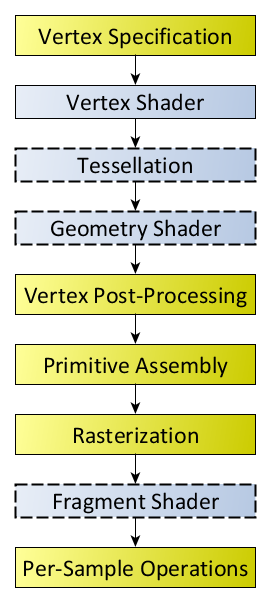
\includegraphics[height=0.75\linewidth]{images/RenderingPipeline.png}
    \caption{Diagram of the Rendering Pipeline. The blue boxes are programmable shader stages
    \cite{openglwiki-rendering-pipeline}.}
    \label{fig:rendering-pipeline}
\end{figure}

\subsubsection{The OpenGL Shading Language}
OpenGL shaders are written in a specialized C-like programming language: OpenGL Shading
Language (GLSL). GLSL has most of the well-known C constructs like branching, loops, functions, etc.
It shares the basic type system but builds on top of it with easy-to-use vectors and matrices \cite{openglwiki-glsl}.
These are used extensively in graphics computations.

Shaders that are integrated into the rendering pipeline also have predefined built-in variables, which
are used to pass data between the pipeline stages \cite{learnopengl-triangle}. Some are mandatory, like the Vertex Shader
\verb|gl_Position| output, while others provide optional flexibility in computation, e.g., the
\verb|gl_Piontsize| output \cite{openglwiki-vertex-shader}.

Another crucial part of the GLSL is uniform variables. The explanation of the uniform storage qualifier
from the OpenGL wiki states that uniforms are global values stored in a program object. Unlike
shader inputs and outputs, they do not change between shader executions, thus making them
uniform \cite{openglwiki-uniform}. While this explanation clearly outlines the core concept behind uniform variables, from
the point of view of an OpenGL beginner, it does a poor job of underlining their importance.
Uniforms allow developers to change the global state within a shader program without the need for
recompilation. For example, uniforms make it possible to adjust the rendered image based on the
camera position for each frame without much overhead.

\subsection{Vertex Processing}
The first stage of the OpenGL rendering pipeline is Vertex Processing. This part of the pipeline takes
as an input a sequence of vertex attributes, such as positions, normals, and texture coordinates,
defined by the user in CPU code. These are then processed via the Vertex Processing sub-stages,
many of which are optional. The output of this stage is vertex data that is passed
on to the Vertex Post-Processing stage \cite{openglwiki-vertex-processing}.

\subsubsection{Vertex Shader}
The first programmable stage of the OpenGL rendering pipeline is the Vertex Shader. It acts on
the vertex data received by the Vertex Processing stage. The Vertex Shader is executed on every
single vertex in the input data in parallel. The OpenGL Wiki states: \enquote{There must be a 1:1 mapping from
input vertices to output vertices.} \cite{openglwiki-vertex-shader}.
This makes it clear that the purpose of the Vertex Shader is to
transform individual vertices without modifying the overall number of them.

The usual way to utilize the Vertex Shader is to apply a series of transformations to the incoming vertex data.
These transformations are carried out as matrix multiplications.
They effectively move the data across a succession of coordinate systems. This is done to emulate the notion of a camera
\cite[p.125-126]{opengl-book}. For simplicity, this section will consider only the transformations of vertex positions,
although there are usually more vertex attributes.

The initial coordinate system is called local (or object) space.
The positions stored in vertex buffers are in this space.
The coordinates are relative to the object's origin, usually its center. For example, vertex positions
representing a square with a side length of 1 could look like this: $[-0.5,-0.5,0], [0.5,-0.5,0], [0.5,0.5,0], [-0.5,0.5,0]$
\cite{learnopengl-coord-systems}.

The next coordinate system to which the vertex positions are transformed is world space.
This is done by multiplying local space positions with the model matrix.
World space intuitively represents the physical space of a scene. World space coordinates
determine an object's location relative to the world origin.
The model matrix encapsulates all the transformations applied to an object to get it from local
to world space. These are translation, rotation, and scaling \cite{learnopengl-coord-systems}.

From world space, the vertex positions are transformed to view space using the view matrix.
The coordinates in view space are relative to the position and orientation of the
simulated camera. The transformation to view space involves translation and rotation \cite{learnopengl-coord-systems}.

The final coordinate system is clip space, and the corresponding matrix is the projection matrix.
This transformation manipulates the view space coordinates in such a way that all vertex positions
that should be visible are mapped to the range of $[-1, 1]$.
Clip space can be described by two parallel rectangular planes perpendicular to the camera orientation vector.
These are referred to as near plane and far plane. The near plane can be thought of as a screen onto which the 3D space is projected.
The far plane limits the visible distance. These two planes form a viewing volume that encompasses all visible objects.
This volume is visualized in Figures \ref{fig:orthographic-frustum} and \ref{fig:perspective-frustum}.
Its shape depends on the type of projection used.
There are two main types of projection. The first is orthographic projection. In this case, the near and far planes
are the same size, and the viewing volume is a prism. The downside of this projection is that it does not take into account
perspective, making it unrealistic. This problem is solved by using perspective projection.
This creates the effect of objects appearing smaller the further they are from the camera.
\begin{figure}[H]
    \centering
    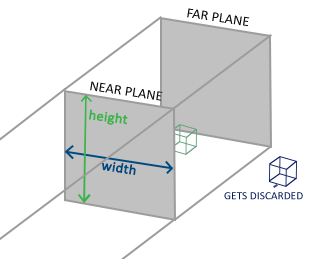
\includegraphics[width=.5\textwidth]{images/orthographic_frustum.png}
    \caption{Orthographic frustum \cite{learnopengl-coord-systems}.}
    \label{fig:orthographic-frustum}
\end{figure}
\begin{figure}[H]
    \centering
    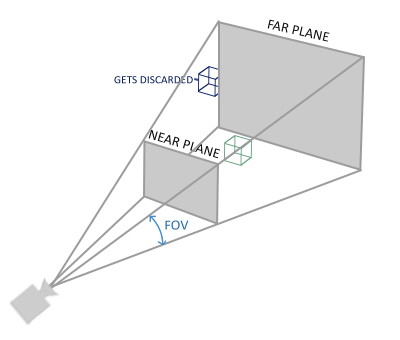
\includegraphics[width=.5\textwidth]{images/perspective_frustum.png}
    \caption{Perspective frustum \cite{learnopengl-coord-systems}.}
    \label{fig:perspective-frustum}
\end{figure}

The clip space vertex positions are then passed to the following stages via the
built-in \verb|gl_Position| variable \cite{openglwiki-vertex-shader}. The following is an example
of a basic Vertex Shader\footnote{Lines beginning with "//" are comments}.
\pagebreak
\begin{minted}{glsl}
// Specify the OpenGL version, in this case it is 3.3.
#version 330 core
// Declare vertex position as an input. This data
// is read from the currently bound vertex buffer.
layout(location = 0) in vec3 pos;
// Declare the model, view, and projection matrix uniforms.
// These are usually set on each frame.
uniform mat4 model;
uniform mat4 view;
uniform mat4 projection;
// The main method is the entry point of execution.
void main() {
  // Transform the object space vertex position using
  // matrix multiplication to clip space. Store the result
  // in the built-in output position variable.
  gl_Position = projection * view * model * vec4(pos, 1.);
}
\end{minted}

\subsubsection{Tessellation}
In the context of the OpenGL rendering pipeline, tessellation is the process of subdividing groups of
vertices referred to as patches into smaller primitives \cite{openglwiki-tessellation}. Therefore, tessellation
can be used to dynamically add detail to meshes, making them look more realistic while keeping
the cost of computation and memory low. A deeper exploration of tessellation and
its use cases is included in Appendix~\ref{app:tessellation}.

\subsubsection{Geometry Shader}
The next stage in the OpenGL rendering pipeline is the Geometry shader. It takes place after the
Vertex Shader (or the optional tessellation shaders) and is the last part of the Vertex Processing
stage in the rendering pipeline. The Geometry Shader offers another optional point of customization
in the rendering process. It takes as input a set of vertices forming a primitive. These primitives can
be points, lines, or triangles. The Geometry Shader can then modify the vertices, add new ones, or
even discard them. Therefore, it can provide a simpler tessellation-like functionality. It then outputs
a set of primitives of the following types: points, line strips, or triangle strips. It is important to note
that the input type does not have to match the output type. Consequently, the Geometry Shader can
completely change the structure of the rendered objects \cite{learnopengl-geometry}\cite{openglwiki-geometry}.

\subsection{Vertex Post-Processing}
Unsurprisingly, after the Vertex Processing stage comes Vertex Post-Processing. This stage takes as an input
the vertex data provided by the last operation in the Vertex Processing stage, i.e., the vertex, tessellation, or geometry shader.
Most of the computations in this stage are handled by fixed-function transformations. That is because the purpose
of Vertex Post-Processing is essentially to prepare incoming data for the next stages of the pipeline, such as Primitive Assembly
and Rasterization \cite{openglwiki-vertex-post-processing}.

\subsubsection{Transform Feedback}
The first part of the Vertex Post-Processing stage is Transform Feedback. It is an optional stage.
Therefore, it has to be explicitly switched on to be active. Furthermore, the computation
performed in this stage cannot be specified to the same extent as in the customizable stages, such as by a shader program.
However, it can be influenced by changing the state of the OpenGL state machine. For example,
the number of captured output variables can be specified
by calling the \verb|glTransformFeedbackVaryings()| function \cite{openglwiki-transform-feedback}.

Transform Feedback is the process of intercepting vertex data transformed by previous stages
in the rendering pipeline (i.e., Vertex, Tessellation, or Geometry shaders) and redirecting it
back into a vertex buffer on the GPU \cite{openglwiki-transform-feedback}. A fascinating use case
of Transform Feedback relevant to modern graphics is explored in detail in Appendix~\ref{app:transform-feedback}.

\subsection{Primitive Assembly}
The next stage in the OpenGL rendering pipeline is Primitive Assembly.
Primitive Assembly is a process of dividing incoming vertex data organized into primitives into a sequence
of base primitives. For example, suppose a drawing command was issued that produced a line strip sequence of 12 vertices.
Because each pair of neighboring points in a line strip represents a line, the Primitive Assembly stage will output
11 line base primitives \cite{openglwiki-primitive-assembly}.

The vertices' coordinates sent to this stage are in clip space (sent via \verb|gl_Position|) \cite{openglwiki-vertex-post-processing}.
This means that all coordinates of vertices that end up being visible on the screen are in the range of $[-1,1]$
\cite{learnopengl-coord-systems}. Clipping, a processing stage within Primitive Assembly, disposes of
parts of incoming primitives lying outside the visible volume. Any primitives positioned solely outside the range
are discarded. Primitives stretching across the boundary may be split, or \enquote{clipped}, into multiple primitives
that fit in the viewing volume \cite[p.12]{opengl-book}.

After clipping, vertex coordinates are transformed using perspective division.
When using perspective projection in the Vertex Processing stages, this step makes objects that are
further away from the projection plane appear smaller. If orthographic projection is employed,
perspective division does nothing.
Then, viewport transformation is applied, mapping coordinates
into the active viewport in window space \cite[p.12]{opengl-book}.

\subsubsection{Face Culling}
The last step of the Primitive Assembly stage is Face Culling. This is an optional stage and
it can be enabled by calling \verb|glEnable(GL_CULL_FACE)|.
If Face Culling is enabled, incoming triangle primitives are discarded based on whether they are facing toward or away from the camera.
The default behavior is discarding back-facing triangles, but it can be overridden \cite{openglwiki-face-culling}.

To determine whether a triangle is front-facing or back-facing, a winding order is introduced. All triangle primitives
are specified by three vertices, the order in which these vertices appear (e.g., in a vertex buffer),
clockwise or counterclockwise, is the winding order \cite{openglwiki-face-culling}\cite{tizen-face-culling}.

Then, the processed triangle primitives are categorized as back-facing or front-facing based on the apparent
winding of the triangle vertices in window space. This is best described by Figure \ref{fig:tizen-front-back-face}
from the Tizen Docs \cite{tizen-face-culling}. The Figure demonstrates how the determinant
is used to calculate the signed area of a triangle. Negative sign indicates CW winding,
positive is CCW.

\begin{figure}[H]
    \centering
    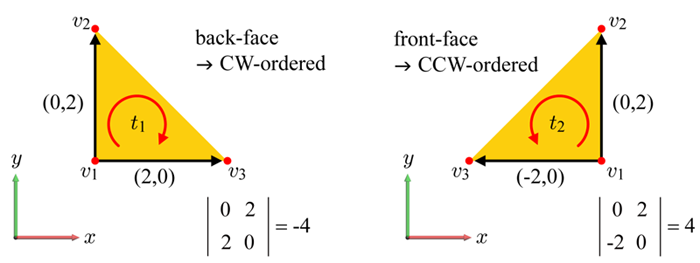
\includegraphics[height=0.32\linewidth]{images/tizen_front_back_face.png}
    \caption{Winding order -- categorizing front/back-facing triangles \cite{tizen-face-culling}}
    \label{fig:tizen-front-back-face}
\end{figure}

\subsection{Rasterization}
After Primitive Assembly, the next stage in the pipeline is Rasterization. At this point, the incoming vertex data
has already been clipped and transformed to window space by the Primitive Assembly stage. Now, it is the Rasterizer's
job to turn the primitives into fragments, each corresponding to a pixel in the framebuffer\footnote{In its simplest
form, a framebuffer contains a grid of pixels that can be displayed on a screen. More on that in
Section~\ref{sec:per-fragment-operations}.} \cite[p.14]{opengl-book}.

A crucial step in the Rasterization process is vertex attribute interpolation. A fragment's calculated attributes
may be influenced by the attributes of all the vertices making up the primitive to which it belongs.
The way the attributes are interpolated can be specified by interpolation qualifiers in the Fragment Shader,
which will be introduced in the next section. There are three basic interpolation qualifiers:
\begin{itemize}
    \item Flat -- The value is not interpolated. All fragments take on the value of the provoking vertex
    in the primitive\footnote{Each primitive contains a single provoking vertex.
    The placement of the provoking vertex in the vertex stream is predetermined by the primitive type.}.
    \item Noperspective -- The value is linearly interpolated in window space.
    \item Smooth -- The value is interpolated correctly with respect to perspective.
\end{itemize}
The Smooth qualifier is set by default and is the right choice most of the time. It allows for seamless
fragment position and texture coordinate calculation \cite{openglwiki-interpolation}.

\subsection{Fragment Processing}
The last programmable stage in the OpenGL rendering pipeline is Fragment Processing.
This stage consists of just the Fragment Shader. Although most implementations of the rendering pipeline function
without a custom Fragment Shader, the default behavior is essentially useless. Therefore, this section will
operate under the assumption that a user-defined Fragment Shader is present.

The Fragment Shader is executed at most once for each fragment generated by the Rasterizer\footnote{The fragment
can be discarded by an early depth or stencil test. In that case, the Fragment Shader is not executed.}.
There are various built-in inputs to the Fragment Shader. However, they are not needed for basic usage of the
Fragment Shader as presented in this thesis. The most useful inputs are user-defined varying variables,
such as world position, normal, and tangent. These are interpolated as explained in the previous section.

The Fragment Shader, in its simplest form, sets the final fragment color. The following is an example
of a basic Fragment Shader that sets the four-component color of its fragment.
\begin{minted}{glsl}
// Specify the OpenGL version
#version 330 core
// Declare the Fragment Shader output variable.
// In this case, it is the fragment color.
out vec4 fragColor;
// The main function is the entry point for execution.
void main() {
  // Set the output variable to a constant color value.
  fragColor = vec4(0.2, 0.8, 1., 1.);
}
\end{minted}

The bulk of the computation performed in Fragment Shaders is often approximating light interactions at objects' surfaces.
The methods used for these calculations will be explored in the following Chapter~\ref{chap:lighting}.

\subsection{Per-Fragment Operations}\label{sec:per-fragment-operations}
Before diving into Per-Fragment Operations, it is crucial to understand the concept of a framebuffer.
At its core, a framebuffer is used to store 2D arrays of pixel data that can later be displayed on the screen.
This data can consist of color, depth, and stencil values. However, more data can be added using framebuffer
attachments. There is a default framebuffer provided by the system, which facilitates drawing to the screen by default \cite{opengl-spec}.

The final stage of the OpenGL rendering pipeline before pixels can appear on a screen is Per-Fragment Operations.
At this point, the fragment data necessary for
rendering has been generated by the preceding Fragment Shader. In this stage, several optional steps operate
on the incoming fragments before storing them as pixels in a frame buffer.
These can be enabled or disabled by changing the OpenGL state \cite[p.46]{opengl-superbible}.

The first operation is the Scissor Test. It can discard fragments that do not belong to a specified rectangular area.
After that, the Stencil Test takes place. It is only executed if there is a stencil buffer attached to
the current framebuffer. A fragment may be discarded based on the comparison of its stencil value
to the value present in the stencil buffer. Depending on the result, the stencil value in the buffer
may be modified. Both the comparison and modification functions are specifiable by the user
\cite[p.504-506]{opengl-book}.

The next operation is the Depth Buffer Test. If there is a depth buffer attached to the current framebuffer,
it keeps track of the distance between pixels and the viewing plane. Each fragment's depth value
is compared to the value in the depth buffer. If the test passes, the value is overwritten.
Typically, fragments further from the viewing plane are discarded. However,
a different comparison function may be selected by the user \cite[p.510]{opengl-book}.

The last notable operation is Blending. After a fragment passes all the previous tests,
its color is written into the framebuffer. However, if blending is enabled,
the fragment color is combined with the existing pixel color.
Both the operation with which the values are combined and the ratios of their contributions
may be specified by the user. A typical use case of blending is rendering translucent objects such as glass \cite[p.251-256]{opengl-book}.

\chapter{Materials}\label{chap:materials}
Shaders are an incredibly powerful tool, but by themselves, they do not provide the best user experience.
That is why modern game engines provide a layer of abstraction on top of shaders called materials.

The Unreal Engine documentation website \cite{ue-materials} introduces the concept of materials with
a simple explanation: \enquote{In the broadest sense, you can think of a Material as the \enquote{paint} that is applied to a mesh
to control its visual appearance.} To be exact, materials dictate how objects' surfaces interact with light sources
in a rendered scene. This sounds a lot like what shaders are used for. The problem that materials solve is best illustrated
by an example.

Imagine rendering a scene displaying a game of pool. On the pool table, there are many balls.
They all have the same physical properties. The only difference is in their color.
If one would use shaders directly to render the objects, sixteen separate
shaders executing almost the same computation would need to be created to display just a couple of balls on a table.
This approach has enormous deficiencies in both usability and performance.
The material layer of abstraction solves this problem by allowing users to parameterize shaders,
thus making them reusable across objects with similar physical properties. With this in mind, instead of creating sixteen
complex lighting shaders, a single shader is referenced by sixteen lightweight materials, each storing its own value
of the shader parameter -- in this case, the color.

After reading the previous sections about shaders, it should come as no surprise that behind the scenes,
shader parameters are actually just uniform variables. These are then simply set by materials when rendering.

Materials are a vital part of modern game engines. Therefore, as a part of this thesis, materials have also been added to AGE.
They can be accessed using the \textit{MaterialSystem} library located in the \textit{gfx} module.

\chapter{Lighting}\label{chap:lighting}
Lighting is a crucial aspect of modern graphics. The nature of the chosen lighting algorithm can vastly impact
the quality of the rendered scene. This thesis implements two approaches to lighting: Phong Lighting and
Physically Based Rendering.

In the real world, the color of a physical surface, as the human eye perceives it, depends on the
energy distribution of photons reaching the retina. These photons may be emitted by multiple light sources.
When a photon reaches a surface, it is either absorbed, refracted, or reflected.
The character of these interactions is determined by the physical properties of the surface.
Simulating the exact physics of real-world lighting is currently not possible. Therefore,
modern lighting algorithms simply aim to approximate it \cite[p.207]{opengl-book}.

\section{Phong Lighting}
The first lighting algorithm implemented in this thesis is Phong Lighting.
It approximates light by splitting it into three components.

The first is ambient. Ambient illumination represents the light that has been scattered
in a scene to a degree that it is impossible to determine its direction and origin.
Adding ambient lighting to a scene results in all surfaces being slightly visible,
even if they are not directly exposed
to light sources. Without it, they would be completely dark \cite[p.208]{opengl-book}.

The next light component is diffuse light. This tends to be the most significant light component.
It is the light that comes from a specific direction, and when reaching the surface,
it scatters uniformly in all directions. The extent to which diffuse lighting affects
a surface's color depends on the angle between the light's direction and the surface's normal.
This angle is illustrated in Figure \ref{fig:diffuse}. As the angle decreases,
the diffuse light's contribution increases \cite{phong}\cite[p.208]{opengl-book}.
\begin{figure}[H]
    \centering
    
\includegraphics[width=0.5\textwidth]{images/diffuse_light.png}
    \caption{Diffuse light calculation \cite{learnopengl-lighting}.}
    \label{fig:diffuse}
\end{figure}

The last component of the Phong Lighting model is specular light.
Similar to diffuse light, specular light comes from a specific direction.
However, unlike diffuse light, it has a preferred reflection direction.
Therefore, this component also depends on the viewing angle relative to the surface.
The more the light's preferred reflection and the camera are aligned, the
more significant the specular light is. All the components necessary for this
computation are depicted in Figure \ref{fig:specular} \cite{phong}\cite[p.208]{opengl-book}.
\begin{figure}[H]
    \centering
    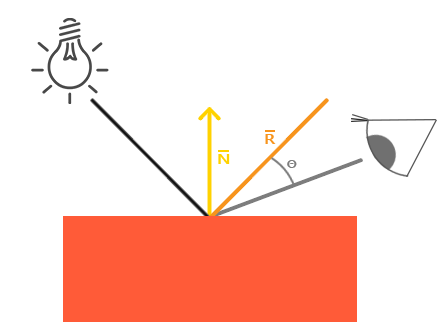
\includegraphics[width=0.5\textwidth]{images/specular_light.png}
    \caption{Specular light calculation \cite{learnopengl-lighting}.}
    \label{fig:specular}
\end{figure}

After calculating all the light's components, the results are multiplied by the light's color.
Then, to apply the light to a surface, the individual light components are multiplied
by the corresponding material color components, i.e., material ambient, diffuse, and specular colors.

\section{Physically Based Rendering}
A modern alternative to the Phong Lighting model is Physically Based Rendering (PBR).
PBR is a lighting model that is designed to closely mimic light's behavior in the real world.
There are several advantages to utilizing the PBR model instead of Phong Lighting and other
non-physically based models. Firstly, materials created with PBR look correct regardless
of the lighting conditions, whereas Phong materials do not. Secondly, artists can create
materials by defining their physical properties instead of relying on their intuition \cite{learnopengl-pbr}\cite{ue-pbr}.

PBR is based on the microfacet surface model. The idea is that rough surfaces can be represented
as comprising many small surfaces, or microfacets, with differing normals. The normals
are modeled by a statistical distribution, and their variance is determined by the roughness of the surface,
i.e., as the roughness increases, so does the variance.
Light's interaction with these microfacets depends on the chosen microfacet model. Usually, they
are treated as perfect mirrors \cite{pbr-book-microfacet}.

The PBR model has several customization points, thus lending itself to highly divergent implementations.
This thesis utilizes the PBR model developed by Epic Games
for Unreal Engine 4 as described by Brian Karis in his SIGGRAPH presentation: Real Shading in
Unreal Engine 4 \cite{ue-real-shading}.

This thesis primarily focuses on shader graphs as a tool for material creation.
Therefore, the underlying mathematics of PBR and the specifics of its implementation are out of the scope
of this thesis. Instead, this section will prioritize the PBR material model, which is more
directly reflected in the shader graph.

The first major difference between the Phong and PBR material models is that there is only one base color component.
Ambient light does not exist in PBR, so material ambient color is pointless. Furthermore, specular color is not
present either. Nevertheless, some PBR material models use specular as a scalar value. However, Unreal Engine 4's
model does not. Brian Karis's presentation \cite{ue-real-shading} explains that the specular parameter
was often misused and that material roughness should be utilized instead. As mentioned before, roughness controls
how much the surface microfacets' normals vary. Higher roughness causes greater light diffusion. On the other
hand, lower roughness results in prominent specular highlights. This effect is illustrated in Figure~\ref{fig:roughness}.
\begin{figure}[H]
    \centering
    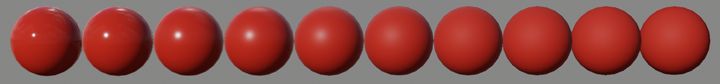
\includegraphics[width=\textwidth]{images/roughness_nonmetal.png}
    
\includegraphics[width=\textwidth]{images/roughness_metal.png}
    \caption{Roughness values from 0 to 1. Nonmetal top, metal bottom \cite{ue-pbr}.}
    \label{fig:roughness}
\end{figure}

Another crucial parameter of the PBR material model is metallic.
It determines whether a material behaves as a metal or a dielectric.
To achieve realism, it should predominately be treated as a binary parameter \cite{ue-pbr}.
The effect of the metallic parameter is illustrated in Figure~\ref{fig:metallic}.
\begin{figure}[H]
    \centering
    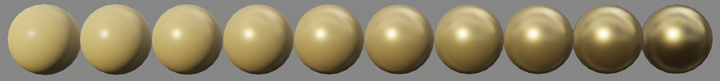
\includegraphics[width=\textwidth]{images/metallic.png}
    \caption{Metallic values from 0 (dielectric) to 1 (metal) \cite{ue-pbr}.}
    \label{fig:metallic}
\end{figure}

The last material property is cavity. This was eventually replaced by the ambient occlusion parameter,
which plays a similar role. Therefore, this thesis will use ambient occlusion instead of cavity.
Ambient occlusion is used to simulate shadows present in small crevices or seams in a surface
\cite{ue-real-shading}\cite{ue-material-inputs}.

\chapter{Shader Graph}\label{chap:shader-graph}
Having gone through the individual stages of the OpenGL rendering pipeline, it is clear that the process of creating and using
shaders in OpenGL has a steep learning curve. Therefore, for the average game designer,
the approach of manually writing shader code to create materials is very impractical.
For this reason, contemporary game engines,
such as Unreal Engine, Unity, and Godot, provide an alternative solution, which is commonly referred to as a shader graph.

Shader graphs empower game engine users to create a wide spectrum of visual effects without having to write a single
line of shader code. Instead of writing code, users can create desired effects visually using a graph-based editor
\cite{unity-shader-graph}. However, this approach also comes with a downside. The Godot documentation website
\cite{godot-visual-shaders} states that visual shaders provide only a subset of shader features.
With higher abstraction and a lack of low-level control, shader graphs have gaps that can only be filled
by writing shaders manually. And that is, in most cases, acceptable. After all, shader graphs simply
aim to fill the use case of approximating light's interaction with a surface.

Shader graphs in modern game engines share a few core concepts. A shader graph loosely follows the structure of
a directed acyclic graph. It consists of nodes with clearly defined input and output slots.
Each output slot can be connected to multiple input slots, providing component reusability.
On the other hand, each input slot may be connected only once. These connections symbolize the flow of data
throughout a shader program. In most shader graphs, there is a single \enquote{output} node.
All data coming from the other nodes is collected there. The inputs of the \enquote{output} node represent the properties
of the resulting material (e.g., color, vertex position).

\section{Shader Graphs in Game Engines}
Before diving into the implementation of the AGE shader graph, it is essential to get an overview of the existing solutions
provided by popular modern game engines. According to the SlashData survey \cite{slashdata-game-engines},
the most popular game engines in order are Unity, Unreal Engine, and Godot. All these engines are equipped with
their own unique versions of the shader graph. Since not all the source code is publicly
available, this thesis explores the shader graphs purely from a user's perspective.

All the game engines featured in this text provide tools for 2D game development. This includes separate versions
of shader graphs for 2D effects and lighting. Nevertheless, because AGE is primarily a 3D game engine, this thesis
will examine 3D graphics shader graph features. Regardless, creating a 2D game is still possible.
That being said, adding quality-of-life features for 2D game development is an opportunity
for future development in AGE.

\subsection{Unity}\label{sec:unity}
The first game engine to explore is Unity. Unity is the most popular game engine in the world \cite{slashdata-game-engines}.
It serves as an excellent introduction to the shader graph concept.

The Unity Shader Graph is available in combination with pipelines derived from the Scriptable Rendering Pipeline (SRP).
These are the Universal Rendering Pipeline (URP) and the High Definition Rendering Pipeline (HDRP) \cite{unity-srp}.
URP is the recommended pipeline for quick and easy development for a broad spectrum of platforms and computing capabilities
\cite{unity-urp}. On the other hand, HDRP is best suited for developing advanced graphics targeting high-end platforms.
It is used for creating AAA games and demands significant computational power \cite{unity-hdrp}.
The choice of the rendering pipeline determines the options and inputs available in the shader graph.
The main focus of this section will be on the shader graph packaged with the Universal Pipeline because of its versatility
and lightweight user experience.

The Unity URP Shader Graph provides multiple material targets in the Graph Settings tab in the Graph Inspector.
These affect the available inputs in the shader graph \cite{unity-graph-settings}. The ones that are relevant
to this thesis are Lit and Unlit.

The main \enquote{output} node of the Unity Shader Graph is referred to by the Unity documentation website
\cite{unity-master-stack} as the Master Stack. It is split into two contexts: Vertex and Fragment,
each representing a stage of a shader program. These contexts contain multiple input slots corresponding
to the final material surface features. The Unlit version of the shader graph consists of the following
inputs: Position, Normal, Tangent, and Base Color. The Lit version then adds properties used for
calculating lighting using the PBR lighting model: Smoothness (the inverse of roughness), Normal (Tangent Space),
Emission, Ambient Occlusion, and Metallic. In the Graph Settings tab, there is an option to switch to a specular material workflow
instead of the default metallic one. When enabled, the Metallic input is replaced by a Specular color input. This allows
the user to specify a different color for specular and diffuse reflections \cite{unity-metallic-specular}.
Transparency and alpha clipping can be enabled in the Graph Settings,
resulting in the addition of the Alpha and Alpha Clip Threshold inputs.

The nodes available in the Unity Shader Graph are listed and categorized in the Node Library section
of the Unity documentation website \cite{unity-node-library}. The top-level categories are Artistic, Channel, Input,
Math, Procedural, Utility, UV, and Block Nodes. Most categories' names speak for themselves; however, some deserve
further clarification. Block node is just a name for the input slots in the Master Stack. Then, there are input nodes,
which belong to perhaps the most useful category. Despite what the name suggests,
input nodes have no input slots, only output slots. Their name is derived from the fact that
they provide input data to other nodes in the shader graph and, subsequently,
to the shader program. They can supply constant values of basic datatypes,
geometry information (e.g., vertex position), scene data (e.g., camera position), and textures \cite{unity-input-nodes}.
Although not included here, parameter nodes can also be considered input nodes.
In Unity, Parameter nodes allow for shader parameterization, a crucial concept covered in Chapter~\ref{chap:materials}.

\subsection{Unreal Engine}\label{sec:unreal-engine}
The next most popular game engine after Unity is Unreal Engine by Epic Games \cite{slashdata-game-engines} dubbed \enquote{The most
powerful real-time 3D creation tool} \cite{ue}.

Similarly to Unity, Unreal Engine's shader graph has a single output node called the Main Material Node \cite{ue-main-node}.
The individual slots on the main node can be enabled or disabled by changing Material Properties in the Details panel. These are
Blend Mode, Shading Model, and Material Domain. Blend Mode controls the alpha blending and masking inputs. The Shading Model
determines light calculations at the material surface. The relevant options are Unlit and Default Lit,
although there are many more interesting options available, such as Hair, Eye, or Cloth. Lastly, the Material Domain
specifies the intended use of the material. For the purpose of this thesis, this will be kept at Surface, meaning that
the created material will be used for lighting calculations at an object's surface \cite{ue-material-inputs}.

In contrast to Unity, Unreal Engine's version of the main output node has quite a few extra input slots. However, many of them
stay disabled based on the chosen Shading Model. When using the Unlit model, only Emissive Color, World Position Offset,
and Pixel Depth Offset are enabled. This implies that Unreal Engine assumes that unlit materials are utilized mostly for rendering lights.
After switching to the Default Lit Shading Model, a considerable amount of inputs become relevant. And because Unreal Engine uses the PBR
lighting model, the newly enabled inputs should be familiar: Base Color, Metallic, Specular, Roughness, Anisotropy,
Normal, Tangent, and Ambient Occlusion. Unlike Unity, Unreal Engine defines the Specular input not as the color of the
specular highlights but as a scalar value determining the amount of reflection at a surface \cite{ue-material-inputs}.

Unreal Engine's shader graph has a colossal Material Expressions\footnote{Material Expressions are what Unreal Engine
calls shader graph nodes.} library. On the Material Expressions Reference website
\cite{ue-expr-reference}, there are 137 nodes listed in a \enquote{reference list of many, but not all, Material Expressions}.
There are a few categories worth mentioning that do not appear in Unity's shader graph. Among them are landscape expressions
for terrain materials, particle expressions, and font expressions.

\subsection{Godot}\label{sec:godot}
The final game engine to explore is Godot. Compared to the other engines covered so far, Godot's documentation
of its version of the shader graph feature is relatively scarce. On the other hand, it partly makes up for it
with its excellent support for writing shaders manually. Nevertheless, a considerable amount of information in this section
is drawn from the actual program rather than the documentation.

As was the case with both Unity and Unreal, Godot's shader graph changes based on the type of shader created.
The only shader type provided by Godot relevant to this thesis is Spatial, which is used for rendering 3D objects
\cite{godot-spatial-shaders}.

Godot named its implementation of the shader graph concept \enquote{Visual Shaders} \cite{godot-visual-shaders}.
In contrast to Unity and Unreal Engine, which share a similar philosophy when it comes to shader graphs,
Godot's Visual Shaders bring a unique perspective. Visual Shaders more closely reflect the underlying
rendering pipeline. To elaborate, the Visual Shader graph is split into three separate graphs:
Vertex, Fragment, and Light. It is clear that the Vertex and Fragment graphs represent data and logic used in the vertex
and Fragment Shader calculations, similar to Unity's contexts.
However, the Light graph provides a feature that is unique to Godot's shader graph.
It allows users to create custom surface lighting. The code from the Lighting shader graph is then incorporated
into the final Fragment Shader in the background. If the main Light graph node is untouched,
Godot defaults to predefined PBR lighting code \cite{godot-shaders-intro}.

Because the vertex and Fragment Shader graphs are separated, data cannot be seamlessly shared between the stages.
In order to share data between stages, varying variables must be used. For that reason, Godot provides
VaryingGetter and VaryingSetter nodes. As for the other nodes in Godot's library, there is nothing standing
out from the other engines.

\chapter{The Academic Game Engine}
The Academic Game Engine (AGE) is an academic project created at the Department of Visual Informatics
at FI MU. At the moment, AGE is in the early stage of development. It serves as a playground for students
of the Game Development study program and a platform for writing theses such as this one.

AGE is split into multiple repositories.
The AGE Data repository contains assets useful for creating games, such as textures and fonts.
The AGE Maker repository provides an application for building scenes. Finally, the AGE Libraries
repository is organized into modules that are comprised of libraries. The following is a brief overview
of the available modules.
\begin{itemize}
    \item \textit{com} -- defines the AGE Context and the structure of the common public interface.
    \item \textit{gfx} -- provides functionality for rendering. The majority of the implementation of this thesis
    took place in this module.
    \item \textit{lfs} -- includes an asynchronous file loader.
    \item \textit{math} -- provides math utilities commonly used in game development.
    \item \textit{osi} -- facilitates user input, windowing, and other system services.
    \item \textit{script} -- serves as a baseline for a future scripting engine.
    \item \textit{utils} -- includes development utilities such as logging and assertions.
\end{itemize}

When creating a game or any other graphics application with AGE, the AGE repositories can be included as submodules
in the main application's repository. This process is best described by the AGE App Template repository's
\textit{README} \cite{age-app-template-readme}. It was also used to create the application
showcasing the functionality created as a part of this thesis (see Appendix~\ref{app:attachments}).

AGE is written in C++ and built using the CMake build system. It utilizes many technologies. However,
the ones relevant to this thesis, i.e., the ones used for rendering, are OpenGL, SDL2 \cite{sdl}, and Glad \cite{glad}.
A brief description of these technologies is included in Appendix~\ref{app:sdl-glad}.

\section{Context}
All of AGE's modules and data exist and operate within the Context.
The Context is a tree data structure that can be thought of as a virtual in-memory disk.
The Context itself is also a library \cite{age-app-template-readme}.
It is the core principle behind AGE. All applications developed with AGE should
exist as a part of it.

The Context is implemented in the \textit{com} module in the AGE Libraries repository.
Before delving into the specifics, it is imperative to highlight that the whole AGE project
uses object-oriented programming principles. The majority
of the disk interface is defined in the \textit{context.hpp} header file. There resides the \textit{ContextItem}
class. It serves as a base class for all objects in the Context. It encompasses the basic
properties of file system objects, such as a name, a path, and a parent folder. There are three classes
that inherit directly from \textit{ContextItem}. The first is \textit{File}, which represents a regular
file. The second is \textit{Folder}. Unsurprisingly, this class mirrors the functionality of folders
in file systems. Its instances can contain other Context objects, thus forming a hierarchy.
A single root folder should be created at the start of the application. Lastly, there is the \textit{Link}
class. Its instances form a symbolic link-like object. Links are basically pointers to other context items
on the disk.

There are two more noteworthy classes used throughout AGE. The first is \textit{Library}. It inherits from
\textit{File}. It is the base class for all AGE Libraries. These are usually instantiated once
and made globally available, thus exposing their interface. The second class is \textit{Runner}. It also
inherits from \textit{File}. Its instances contain instructions that should be executed
in each iteration of the main application loop, such as rendering a scene. In the application
attached to this thesis, the main runner is an instance of the \textit{Presenter} class,
which inherits from \textit{Runner}.

Besides the tree-like data structure, the Context is equipped with a built-in event system.
Instances of classes inheriting from \textit{ContextItem},
may register to watch other objects. When the watched object's content changes, the
watching object will be notified with the event information. There are many event-handling
functions available in the base Context classes. They can be overridden
to create custom event callback functions.

\section{Gfx Module}
The main module used for rendering objects in AGE is \textit{gfx}.
This is where the majority of the implementation occurred. Users can interact with the
\textit{gfx} module through its many library objects. As discussed in the previous section,
these are classes inheriting from the \textit{Library} class. There are many
libraries in this module. This section will briefly cover the most essential ones.

Perhaps the most frequently used library in the \textit{gfx} module is the \textit{ObjectSystem}.
It exposes an API for managing objects that can be rendered on a screen.
Objects are stored in the Context as directories containing all the data
necessary for their rendering. This includes vertex data buffers managed by the \textit{BufferSystem} library,
lights operated by the \textit{LightSystem} library, materials overseen by the \textit{MaterialSystem} library,
and finally, frames that hold information about position and rotation in space.
The following is an example structure of such an object in the Context.
\begin{verbatim}
box/
|-- material.link
|-- buffer.link
|-- frames/
|   |-- frame.link
|-- lights/
    |-- directional.link
    |-- point-1.link
    |-- point-2.link
\end{verbatim}


Notice that the object does not contain the data itself. However, it holds references (links) to data managed by other
libraries. This allows for seamless reusability. For example, a directional light may influence many objects
while existing on the disk only once.

Besides the \textit{ObjectSystem}, there are a few more noteworthy libraries in the \textit{gfx} module.
Firstly, there is the \textit{ShaderSystem}, which unsurprisingly facilitates the creation and management
of shaders. In the Context, these are represented as files.
Before the work of this thesis, shaders used to be directly attached to objects.
That means that instead of the \verb|material.link|, there would be a \verb|shader.link|.
However, as explained in Chapter~\ref{chap:materials}, this can lead to complications. Therefore,
the \textit{MaterialSystem} library was introduced as a layer of abstraction between objects and shaders.
Materials are folders containing a reference to a shader file. They also control a folder with uniforms
parameterizing the shader.

The last crucial library in the \textit{gfx} module is the \textit{Renderer}. It will be thoroughly explored
in the following section.

\section{Rendering Pipeline}
Before diving into the implementation of the AGE Shader Graph, it is crucial to understand
the AGE Rendering Pipeline on top of which the shader graph was built.

A substantial amount of time had to be dedicated to implementing the rendering pipeline functionality
necessary for the support of the shader graph's extensive feature set.
Prior to this thesis' contributions,
the pipeline was equipped with only the capability to render objects using their attached shaders
with the forward shading method without integrated lighting. As a part of this thesis, support for multiple lighting models,
deferred shading, and transparency rendering was incorporated, among other features.

The whole rendering pipeline is encapsulated in the \textit{Renderer} library class located
in the \textit{gfx} module. This is perhaps the best-documented library interface in AGE.
Therefore, to gain an understanding of the specifics of the implementation,
I recommend looking at the source code in files \textit{renderer.hpp} and \textit{renderer.cpp}.

For an object to be rendered using the AGE rendering pipeline, it has to comply with a predefined
directory structure, as showcased in the previous section. Consequently, it is recommended to utilize
the \textit{ObjectSystem} library to manage objects instead of manipulating the Context directly.
Besides being more convenient, it also prevents accidental object structure errors.

From a user's perspective, the basic rendering workflow has only two steps that have to be executed on each frame.
Firstly, clear the render buffers by calling \verb|Renderer::clear_render_buffers()|. Secondly, render objects
on the screen using \verb|Renderer::present_collection()|. This function recursively searches through a directory
specified by its first argument using the depth-first-search strategy and renders any objects it encounters.
The function's second argument is the rendering mode. The distinct rendering modes will be explored
in Sections~\ref{sec:forward-mode}-\ref{sec:transparent-mode}.

The rendering of a single object is handled by the \verb|Renderer::|\\
\verb|present_object()| function.
The function is called internally only. Users do not have access to it.
The following is a high-level summary of the steps it takes to display an object on a screen.
\begin{enumerate}
    \item Find the \verb|material.link| and activate its corresponding shader program.
    
    \item Set any per-frame uniforms, such as the camera position,
    view, and projection matrices, etc.

    \item If the active shader program comes from a forward-lit shader, iterate through the \verb|lights/| folder
    and set the uniforms required for lighting calculations (e.g., color, position).

    \item Locate the \verb|buffer.link| and bind the referenced vertex data buffers. These
    can include vertex positions, normals, tangents, etc.

    \item Iterate through the \verb|frames/| folder\footnote{This is not the case when using Transparent mode.}
    and for each frame:

    \begin{enumerate}
        \item[5.1.] Set its position and rotation transformation as the model matrix uniform.
        
        \item[5.2.] Invoke an OpenGL draw function.
    \end{enumerate}
\end{enumerate}
This sequence of steps is taken for each object when rendering a scene. However, it may vary depending
on the chosen rendering mode.

\subsection{Forward Mode}\label{sec:forward-mode}
The first and most straightforward AGE rendering pipeline mode is the Forward mode. It represents the forward shading method.
Forward shading is an intuitive technique that utilizes a single
shader program to compute an object's appearance. The object basically takes a single pass through the OpenGL pipeline.

The steps taken when rendering objects with the Forward mode are identical to the procedure outlined
in the previous section.

\subsection{Deferred Mode}
The second available rendering mode is the Deferred mode. Similar to the Forward mode, it also represents
a rendering technique called deferred shading. In contrast to forward shading, this method is considerably
more complex in terms of implementation.

Before diving into the specifics, it is essential to highlight the problems with forward shading
that deferred shading aims to solve. When using forward shading to render a lit scene,
for each fragment produced by the Rasterizer, the Fragment shader has to compute the contributions
of all light sources to the final fragment color. If the scene is complex, it is likely that on many occasions,
this color is not even used because it is overwritten by another fragment closer to the camera.
This is an enormous waste of computing resources.

Deferred shading tackles this performance problem by postponing (or deferring) the exhaustive lighting computations to a later stage.
Instead of immediately calculating the final color of each fragment,
the idea is to first store all the information necessary for per-fragment lighting
(e.g., normals, material color, etc.) in the GPU's memory. This stage is called the geometry pass. It sounds
simple enough. However, there is a caveat. The intermediate data cannot be rendered into the default framebuffer.
That is because the framebuffer expects to receive a single color value per pixel.
This problem is solved by creating a dedicated geometry framebuffer, called the \emph{gBuffer}, and attaching textures to it
that can store the lighting-relevant data for later use \cite{learnopengl-deferred}.

Besides the lighting data, it is also necessary
to store the depth values to be used in the depth test. This could be accomplished by attaching another texture
to the new framebuffer. However, fragment depth is not relevant to lighting.
Therefore, the depth buffer will only be used for writing data, not reading it\footnote{The depth will not be read by user-defined shaders.
However, it will still be read during the depth test.}. This provides an opportunity for optimization.
Instead of using another texture, a special buffer object called the renderbuffer can be utilized as the new
framebuffer's depth buffer. The advantage of this approach is that, unlike textures, the renderbuffer object is optimized for
use as a render target \cite[p.526-540]{opengl-book} \cite{openglwiki-rbo}.

After the geometry pass has rendered all objects, only the fragments that will become
the final pixels are present in the \emph{gBuffer}. The next step is to compute the final colors of the pixels
and store them in the default framebuffer, thus completing the lighting pass.

The simplest way to execute the lighting pass is by issuing a draw command that renders a single triangle
spanning the whole projection plane in clip space. Then, in the Fragment shader, the lighting can be computed
using the populated \emph{gBuffer} textures. For each pixel, the contribution
of all lights in the scene has to be accounted for. This leads to a time complexity of $\mathcal{O}(P\cdot L)$\footnote{This
does not take into account the geometry pass. However, that is insignificant compared to the time spent calculating lighting.},
where $P$ is the number of pixels, and $L$ is the number of lights in a scene. This is technically
more efficient than forward rendering that has a time complexity of $\mathcal{O}(F\cdot L)$, where $F$
is the number of generated fragments. However, there is a better approach \cite{learnopengl-deferred}.

A point light's influence on a fragment's color diminishes over distance. At some point, the light's
contribution becomes imperceptible on a screen. This distance can be thought of as the light's radius.
Therefore, iterating through all lights for each fragment can lead to a large amount of meaningless computation.
This issue can be addressed by utilizing light volumes. Each point light in a scene is rendered as a sphere
with a radius identical to the light's radius and the light at its center. The sphere's Fragment Shader
then calculates only the light's contributions to pixels inside its radius. This leads
to a time complexity of $\mathcal{O}(P + L)$. The light
volumes must be rendered with blending enabled so that overlapping lights add up \cite{learnopengl-deferred}.

The light volumes render only lighting associated with point lights. For directional lighting,
another lighting pass is executed. This can take the form of the previously mentioned straightforward approach.
Iterating through all lights per pixel is not problematic because there is usually a single directional light per scene.

The deferred shading technique is a great tool for efficiently rendering complex scenes, especially
ones with many lights. However, it does have its drawbacks.
Firstly, some effects, such as alpha blending, cannot be achieved with deferred shading. That is because, by the time
the final pixel color is to be computed, only a single fragment per pixel remains in the \emph{gBuffer}. To achieve
alpha blending in combination with deferred shading, the blended objects have to be rendered separately after
the deferred shading pass, using forward shading. However, this requires copying the renderbuffer object's depth
buffer into the default framebuffer's depth buffer in order to perform the depth test correctly. Another
disadvantage of the deferred shading method is the memory and buffer management overhead \cite{learnopengl-deferred}.

In conclusion, deferred shading should only be used when rendering complex scenes with many light sources.
For simple scenes, the disadvantages outweigh the benefits.

Recommended Deferred mode usage is well documented in the \textit{Renderer}'s header file.
Therefore, this section will focus on the inner workings
of the implementation. Before the per-frame operations begin,
the \textit{Renderer} creates the \emph{gBuffer} and all the necessary textures/buffers. Then, on each frame:
\begin{enumerate}
    \item Clear all buffers and \emph{gBuffer} textures.
    
    \item Bind the \emph{gBuffer} as the current framebuffer.
    
    \item Render the objects' data into the \emph{gBuffer}. This follows the same structure as presented in the
    \verb|Renderer::present_object()| function explanation.

    \item Gather all lights associated with the rendered objects\footnote{There is no way to determine
    which pixels should be affected by which lights. Therefore, when rendering a scene with deferred rendering,
    if a light is attached to a single object in the scene, it also affects all other objects.}.

    \item Bind the default framebuffer as the current framebuffer.

    \item Execute the lighting pass using predefined lighting shaders.

    \item (Optional) Copy the \emph{gBuffer}'s depth buffer into the default framebuffer's depth buffer.
\end{enumerate}

\subsection{Transparent Mode}\label{sec:transparent-mode}
The last available rendering mode is the Transparent mode. This mode is dedicated to rendering partially
transparent objects. Unlike the previous mode, the implementation is not nearly as complicated.
Because it utilizes forward shading, it essentially follows the same structure as the Forward mode
but with a few extra steps.

Transparent mode utilizes blending, which was already discussed in Section \ref{sec:per-fragment-operations}.
In this mode, blending is enabled implicitly. However, the \textit{Renderer}'s public interface contains
a blending configuration function, which allows user customization.

Rendering partially transparent objects has its complications. Imagine a simple scene
with two cubes, one positioned behind the other. Suppose
that the front cube is drawn first. If the front cube is opaque, the back cube's
color should not influence the final color. This is correctly prevented by the depth test.
However, if the front cube is partially transparent, both colors should be combined.
In this case, the depth test undesirably discards the back cube fragments.
The solution is first to draw all fully opaque objects with standard forward shading.
Then, the transparent objects are drawn with the depth buffer in read-only mode.
That way, transparent objects obscured by opaque ones are discarded, and all overlapping
transparent objects are rendered \cite[p.263]{opengl-book}. This problem and its solution
are illustrated in Figures \ref{fig:incorrect-alpha} and \ref{fig:correct-alpha} generated by the
attached application.
\begin{figure}[H]
    \centering
    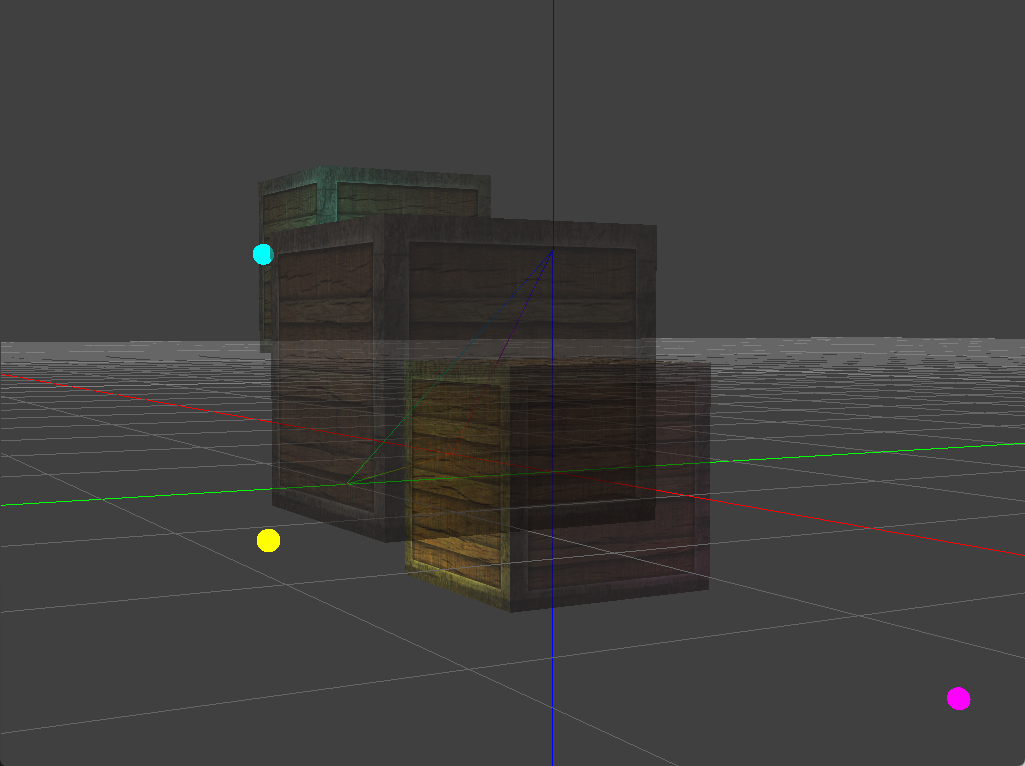
\includegraphics[width=.6\textwidth]{images/incorrect-alpha.png}
    \caption{Blending with depth writing enabled.}
    \label{fig:incorrect-alpha}
\end{figure}
\begin{figure}[H]
    \centering
    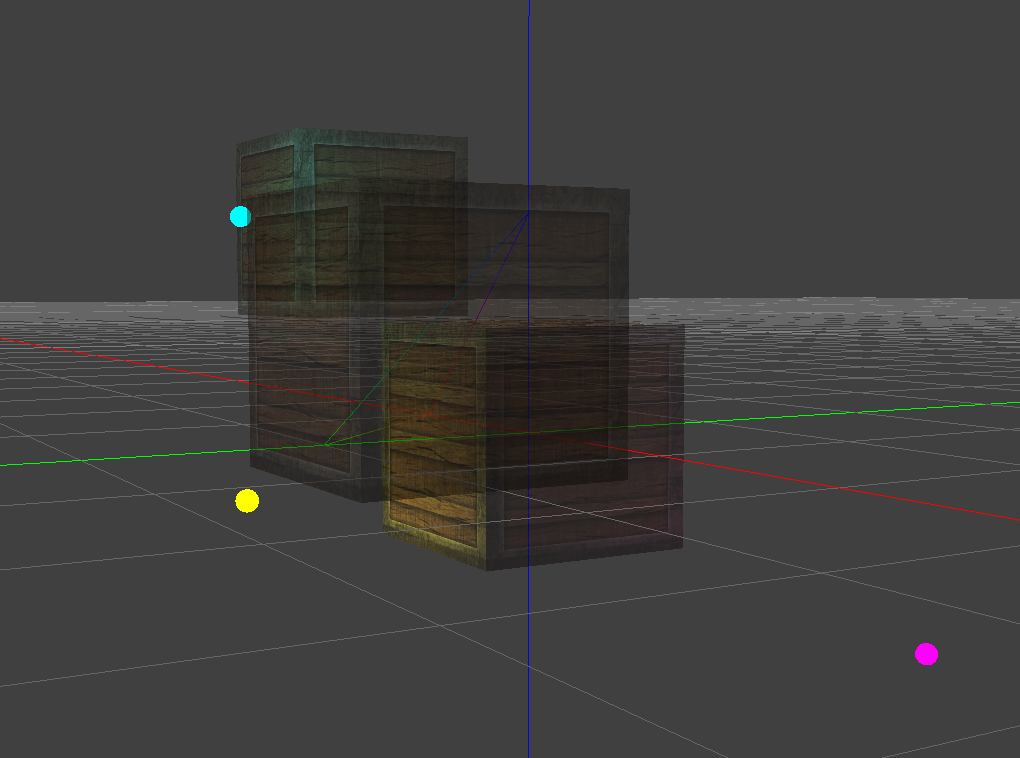
\includegraphics[width=.6\textwidth]{images/correct-alpha.png}
    \caption{Blending with depth writing disabled.}
    \label{fig:correct-alpha}
\end{figure}

The previous paragraph outlined the solution for the interaction of opaque/transparent
objects. However, there is a deeper problem connected to it.
Because of the nature of the OpenGL blending functions, the final color of blended
fragments can vary greatly depending on the order in which they are drawn \cite[p.263]{opengl-book}.
To achieve a realistic render, blended fragments must be drawn in a consistent
order from back to front. This problem does not have a simple solution.
If two or more semi-transparent objects overlap such that some parts of an object are
in front of and some behind the other objects\footnote{This sounds like an edge case that does not occur often.
However, it can happen easily, even in simple scenes. See \cite{alpha-sorting}.},
there is no way to order the fragments correctly.

The AGE rendering pipeline takes a simplistic approach to achieve satisfactory results.
When rendering with the Transparent mode, before any objects are drawn,
all their frames are gathered. Then, the frames are sorted based on the distance
from their origins to the camera. Finally, the frames and their corresponding objects are drawn
from the furthest to the closest.

\chapter{The AGE Shader Graph}
On top of the rendering pipeline foundation stands the AGE Shader Graph module.
In the context of the AGE philosophy, the shader graph is represented as a single file.
The inner workings of the shader code generation logic were conceived without outer inspiration.
In contrast, the design process behind the AGE Shader Graph's public interface was predominantly influenced
by the existing solutions provided by contemporary game engines.

Chapter~\ref{chap:shader-graph} objectively examined the most popular game engines and their unique versions of the shader graph.
The AGE Shader Graph aims to combine the desirable qualities of these shader graphs.
One of the qualities considered in the design is the separation of the main output node into shader stages.
This trait is included in the Godot and Unity game engines. Unity splits its Master Stack's inputs into contexts.
This explicitly determines which inputs belong to which shader stage.
Godot takes this concept further by separating the entire graph into stages. However, this
has a negative impact on user experience as discussed in Section~\ref{sec:godot}.

Section~\ref{sec:unreal-engine} explored the Unreal Engine's version of the shader graph.
This shader graph is clearly equipped with a more extensive feature set. However, it can be
quite overwhelming from a user's perspective. With this is mind, the AGE Shader Graph
took a more simplistic approach providing a beginner-friendly interface.

Besides the designs implemented by other game engines, there was another option to consider.
Prior to this thesis, AGE had an outline
of a shader graph that closely followed the structure of a manually written shader program.
It was essentially the GLSL wrapped into graph nodes. It included constructs
such as loops, if conditions, and built-in shader outputs. This type of shader graph
is undoubtedly more powerful. However, it defeats the primary purpose of the shader graph concept.
That is, quickly creating visual effects while avoiding writing low-level GLSL code.

In conclusion, the AGE Shader Graph took inspiration primarily from the Unity game engine
as opposed to other designs.

\section{Shader Class Hierarchy}
The AGE shaders are organized into a class hierarchy that consists of three classes: \textit{Shader},
\textit{ShaderGraph}, and \textit{TextShader}. Before this thesis, the only type of shader in AGE
was the outline of what would become the \textit{ShaderGraph} class. There are two reasons
behind the creation of the \textit{TextShader} class. Firstly, the Performance Evaluation
portion of this thesis uses manually written shaders to measure the shader graph's relative performance.
Secondly, as mentioned before, shader graphs are inherently
unable to fulfill the whole set of possibilities provided by handwritten shaders. Therefore,
adding the \textit{TextShader} brings a broader spectrum of capabilities to AGE users.

The \textit{Shader} class is the base of the hierarchy defining defines the common interface
with which the \textit{gfx} libraries interact. This includes methods such as shader compilation,
activation, and setting uniforms. The inheriting classes then extend this functionality
and expose it to the user. The \textit{TextShader} class simply offers a mechanism for creating
shaders out of strings. On the other hand, the \textit{ShaderGraph} class comes equipped
with a node library and broad spectrum of tools for shader node creation and manipulation.

\section{Graph Node}
All the nodes in the AGE Shader Graph's node library follow the same pattern outlined
in the \textit{Node} base class. At its core, a shader graph node represents a piece of shader code.
However, from a user's perspective, a node is a black box that takes a collection of values delivered via input slots,
transforms it, and supplies the results via output slots. These slots
can be connected to other nodes' slots, thus forming a shader graph. Each slot has a specific
data type, which mirrors GLSL types.

In AGE, for a pair of slots to be connected, their types have to match.
This is not the case for all shader graphs. Some allow the bending of types.
For example, in Godot, the albedo color input of the main output node has the type of a 3-component vector (\textit{vec3}).
Yet, nodes of all vector, scalar, and even Boolean types can be connected to it. Furthermore, these conversions
have different behaviors. On conversion, a \textit{vec2} is extended to a \textit{vec3} with the third component being zero,
a \textit{vec4} loses its last component, a scalar's value is copied three times to form a \textit{vec3}, and a Boolean is converted
to scalar one or zero and then follows the previous case. Except for the \textit{vec2} conversion,
these are all valid ways to create a \textit{vec3} in the GLSL \cite{openglwiki-datatype}.
This approach can lead to higher flexibility. However, it can also cause a lot of confusion and hidden errors.
For this reason, the AGE Shader Graph implements a strict typing system.

In shader graphs, it is crucial that logic defined in a node or a collection of nodes forms a reusable subgraph.
This is achieved by allowing output slots to be connected to multiple input slots.
While that sounds perfectly reasonable, it will later be shown that it can be quite problematic to implement efficiently.

The AGE Shader Graph can be thought of as
a directed acyclic graph with a single root node called the Master Node. The graph's edges are
directed from input slots towards output slots. The root has no outputs, and the leaves have no inputs.
When compiling a shader graph, the graph is traversed using the DFS 
strategy starting from the root node. Each node overrides the \verb|add_code()| virtual method.
This method is called when visiting a node to generate its piece of shader code.
It is crucial to traverse the graph in postorder so that a node's code is added only after all its input nodes'
code fragments are present.

To inline or not to inline, that is the question. Inlining is an optimization technique
implemented by modern compilers. A function that is to be inlined has all its invocations
replaced by its body. During the shader graph's implementation, a design
decision was made to generate code without any inlining. Consequently, each node in the graph has its own
variable with a unique name declared in the shader code. This variable is then
referenced by any nodes that take the original node as input. On the one hand,
the downside of this approach is that it leads to the creation of many variables consuming memory on the stack.
Even a simple addition of two scalar values is stored in a separate variable. On the other hand,
when a graph contains a component that is reused in many places (i.e., its output is connected to many inputs),
the component's computation is executed only once. An example of a node that performs an expensive
calculation is the matrix multiplication node. Instead of multiplying the same matrices in multiple
places, the computation is performed once and stored in a variable for future use. Furthermore,
this approach allows nodes to generate the same code regardless of what nodes are connected
to their inputs. The predetermined variable names of input nodes are simply plugged into
the node's code fragment.

\section{Master Node}
Except for the main output nodes, all other nodes in the shader graphs explored by Chapter~\ref{chap:shader-graph}
follow practically the same principles that were outlined in the previous section.
The fundamental differences in the graphs lay in their main output nodes. In AGE, this node
is called the Master Node. It has no output slots, and its input slots correspond to the properties
of the chosen material model (see Chapter~\ref{chap:lighting}). The collection of input slots available in the Master Node
determines the set of possible effects achievable by the shader graph.

The AGE Shader Graph has five versions of the Master Node. A single Master Node
is inserted by the graph's constructor based on the constructor's arguments.
The constructor takes four arguments.
\begin{itemize}
    \item Name -- the file name passed to the \textit{ContextItem} constructor.
    \item Lighting -- chooses the shading technique. This can be unlit, forward-lit, or deferred.
    \item Lighting Model -- defaults to Phong but can be set to PBR. It has no effect if the shader is unlit.
    \item Transparency -- defaults to opaque. It can be partial or threshold if the shader does not use
    deferred shading. The transparency options will be briefly explained in the following section.
\end{itemize}

Based on these inputs, a specific Master Node type is selected. The available Master Node types are
Unlit, Lit, Deferred, PBR, and Deferred PBR. Each provides a unique set of input slots.
These inputs are listed and described in the Master Node definitions in the \textit{gfx} module.
They should be self-explanatory after reading Chapter~\ref{chap:lighting}.
Therefore, they will not be redundantly listed in this text.
However, there are some noteworthy input slots that facilitate valuable effects.
Firstly, the transparency input slots provide alpha blending and alpha clipping effects.
These are enabled by selecting the partial and threshold transparency modes respectively.
Secondly, the fragment normal and ambient occlusion input slots accommodate the use of normal and ambient occlusion maps.
These can add surface detail to objects without the overhead of a more detailed mesh.

In the source code, the Master Nodes' input slots are visually separated into two categories:
Vertex and Fragment. Naturally, these represent the shader stages in which the inputs are utilized.
This takes inspiration from the Unity Contexts highlighted in Section~\ref{sec:unity}.
The Vertex inputs facilitate various vertex transformations. However, the more intriguing inputs
belong to the Fragment category. These directly influence how light interacts with an object's surface.
They correspond to the parameters of the two chosen material models depicted in Chapter~\ref{chap:lighting}.

With the Master Node, the AGE Shader Graph aims to provide a set of features
that matches the intersection of the functionality available in the modern shader graphs examined in this thesis.
On top of that, it comes equipped with a built-in Phong lighting shader graph variant, which
is not a standard feature in contemporary game engines.

\section{Node Library}
A shader graph's node library is a collection of nodes used to generate and transform
data in a shader program. Having gone through the node libraries of the Godot, Unity, and Unreal Engine game engines
in Sections \ref{sec:godot}, \ref{sec:unity}, and \ref{sec:unreal-engine},
it is apparent that they provide an obscene amount of nodes\footnote{For example, Unreal Engine's Material Expressions Library comes equipped
with over 130 nodes \cite{ue-expr-reference}.}. On the other hand, AGE's node library implements only essential ones.

Similar to the Godot, Unity, and Unreal Engine node libraries, the AGE node library is split into
categories. The following is a brief overview of the available node categories\footnote{For a more
detailed description of the categories and their corresponding nodes,
consult the \textit{gfx} module header files.}.
\begin{itemize}
    \item Input Nodes -- provide data to the shader program. They include nodes such as Varying Position Node,
    Texture Node, and Uniform Node.
    \item Operator Nodes -- combine one or more inputs with an operator, such as addition, multiplication,
    and subtraction.
    \item Vector Utility Nodes -- are used to convert data between vector and scalar types (e.g., Decompose Vector Node).
    \item Noise Generation Nodes -- act as a source of pseudo-randomness.
    \item Logic Nodes -- their output is based on a Boolean condition.
    \item Math Nodes -- supply standard math functions (e.g., Sine Node).
\end{itemize}

The most complex nodes to implement are the Input Nodes. All other node types simply take their inputs,
transform them in terms of GLSL code, and send the result to their output slots.

\subsection{Input Nodes}
Input Nodes' primary responsibility is to expose data usable by a shader program to the shader graph.
Most Input Nodes do not have any input slots.

Firstly, there is the Uniform Node.
This node is used to parameterize shaders, as explained in Chapter~\ref{chap:materials}.
Uniform Nodes are managed by material instances. Each material has a \verb|uniforms/| folder
containing files with values corresponding to the Uniform Nodes of the referenced shader graph.
Upon material activation, the shader's uniforms are set based on the contents of the uniforms files.

Then, there is the Texture Node. In contrast to other Input Nodes, it has an input slot that accepts texture coordinates.
Texture Nodes are responsible for generating textures from image
files and making them available to the shader program. The files are loaded asynchronously using the
\textit{lfs::Loader} library. After the files are successfully loaded, the AGE event system triggers the texture generation.
Then, during shader activation, each texture is assigned
a texture unit, and its sampler uniforms are set accordingly.

\subsection{Flexibility}\label{sec:flexibility}
Even with a few nodes in the node library, a broad spectrum of effects
is achievable with the AGE Shader Graph. This is demonstrated by the examples showcased
in the attached application. This section will establish the flexibility and effectiveness of
the AGE Shader Graph.

Perhaps the most versatile node in the AGE Shader Graph is the Custom Function Node.
It was designed to allow the user to create
new nodes on-demand with minimal effort. To create a Custom Function Node,
one has to specify the input names and types, the output type,
and the GLSL code that computes the result. This code is then internally wrapped in a function
whose arguments correspond to the given input names and types.
The Custom Function Node is displayed in the Custom Function example in the attached application
and in Appendix~\ref{app:custom-function-node-example}.
There, it is utilized to perform a calculation with nested trigonometric functions,
some of which are not available in the shader graph but are exposed by the GLSL.

Many nodes in modern shader graphs do not add any functionality that is not
attainable without them. They are there to facilitate common use cases
and thus accelerate development. An example of such a node that is present
in all discussed game engines is the remap node. It remaps a value
from some range to a different range. Godot's version of this node can be seen in Figure \ref{fig:godot-remap-node}.
\begin{figure}[H]
    \centering
    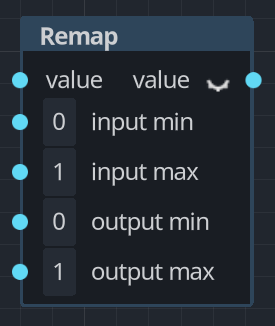
\includegraphics[height=0.3\textwidth]{images/godot_remap_node.png}
    \caption{Godot's Remap Node}
    \label{fig:godot-remap-node}
\end{figure}

Even though this node is not present in AGE's node library, it can be easily recreated.
One possible implementation is demostrated in Appendix~\ref{app:remap-node}.

\subsection{Extensibility}\label{sec:extensibility}
The primary concern with the AGE node library's design is its extensibility.
The node library is currently relatively small. Therefore, it is crucial that more nodes
can easily be added in the future. Apart from Input Nodes, which may require a deeper
understanding of the shader code generation logic, creating new nodes is relatively
simple. The following sequence of steps describes the recommended approach
to node creation.
\begin{enumerate}
    \item Declare a new node class (or struct) in the \textit{ShaderGraph} class namespace
    so that it is accessible through \\\textit{ShaderGraph::NewNodeClass}.
    \item Place the definition of the node class in the shader nodes header file.
    \begin{enumerate}
        \item[2.1.] It should inherit from the base \textit{Node} class or any other
        fitting class in the hierarchy.
        \item[2.2.] Define its constructor by calling the \textit{Node} constructor
        with the node's name, description, and a list of input and output slots.
        This should be done in the header file so all information
        necessary for its usage is available there.
        \item[2.3.] Override the \verb|Node::add_code()| method.
        \item[2.4.] (Optional) If there are input slots
        with distinct meanings\footnote{For example, this would be meaningless
        when creating a simple addition node.}, define an input slot enum
        so that it can be used for indexing input slots instead of integers.
    \end{enumerate}
    \item Place the definition of the overridden \verb|Node::add_code()| method
    in the shader nodes source file.
\end{enumerate}

\chapter{Performance Evaluation}\label{chap:performance-evaluation}
Besides evaluating the AGE Shader Graph based on the set of achievable effects,
it is crucial to consider performance as well. Specifically, the performance of the
generated shaders. For this reason, the \textit{TextShader} class was created.
It serves as a baseline for performance comparison. The primary focus of the evaluation
is the application's frame rate measured in terms of frames per second (FPS).
A secondary metric is the compilation time of the generated shaders.

The measurement results presented in this chapter were generated by a partially automated
process. There are instructions for their reproduction in the \verb|measuring-utils/README.md|
file in the attached repository. The scenes used for benchmarking are also included in the
examples in the attached application.

All measurements were conducted using a Lenovo ThinkPad T14s Gen 2i notebook running on
the Fedora Linux 40 (Workstation Edition) 64-bit operating system.
The notebook has an 11th Gen Intel® Core™ i7-1185G7 × 8 processor and an Intel® Xe Graphics (TGL GT2)
graphics processor.

\section{Frame Rate}
Two separate frame rate metrics were considered in the shader graph's performance
evaluation. These are FPS on the CPU and approximated FPS on the GPU.
The CPU FPS metric corresponds to the frame rate of the whole application.
It is measured via the \textit{osi::Timer} class.
On the other hand, the GPU FPS metric approximates the GPU frame rate by taking into account only time
spent on executing rendering commands. The GPU measurements are handled by the \textit{app::Presenter} class
using OpenGL time queries. Both metrics take into account unstable start-up performance by discarding
data measured during a predetermined number of warm-up iterations.

Tables \ref{tab:fps-comparison-phong} and \ref{tab:fps-comparison-pbr} depict the results of the
measurements of the two metrics. The performance of forward and deferred shaders generated by the
AGE Shader Graph is compared to manually written forward and deferred shaders accomplishing the same exact effect.
The performance is measured across a series of scenes with an increasing number of objects
and point lights. The rows and columns represent the number of boxes and point lights in the scene, respectively.
The cells are conditionally formatted with a gradient. CPU and GPU FPS have separate gradients.
\begin{table}[H]
    \centering
    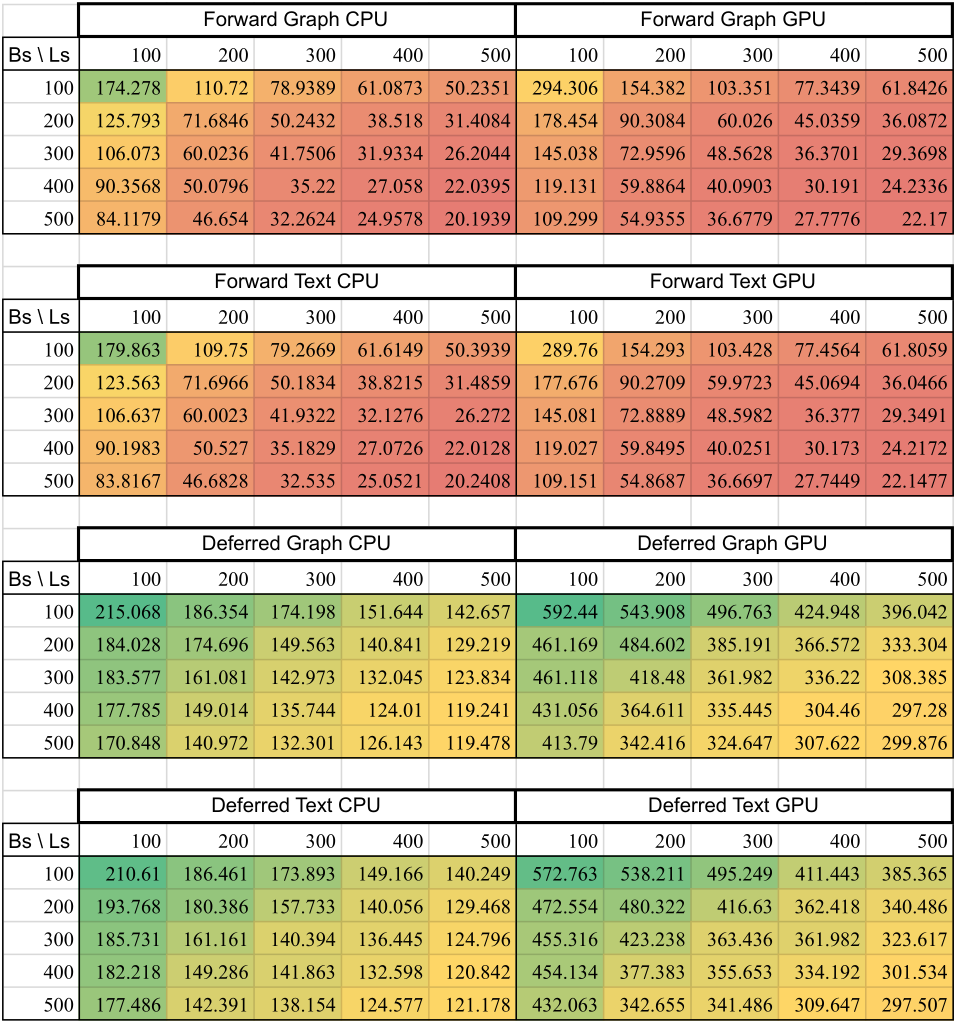
\includegraphics[width=\textwidth]{FPS/MeasureFPSReformat.png}
    \caption{FPS comparison of Phong shader graphs and handwritten shaders}
    \label{tab:fps-comparison-phong}
\end{table}
\begin{table}[H]
    \centering
    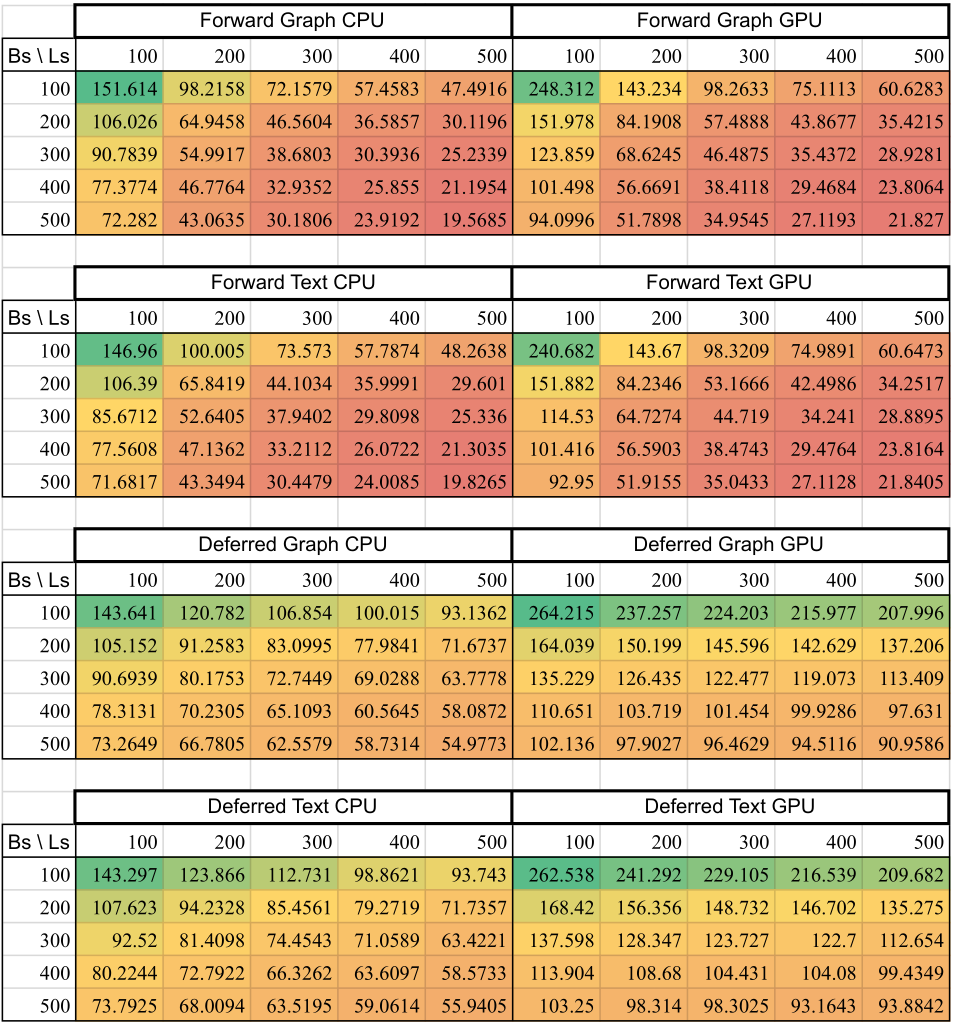
\includegraphics[width=\textwidth]{FPS/MeasureFPS-PBR.png}
    \caption{FPS comparison of PBR shader graphs and handwritten shaders}
    \label{tab:fps-comparison-pbr}
\end{table}

Tables \ref{tab:fps-comparison-phong} and \ref{tab:fps-comparison-pbr} clearly demonstrate that there is no significant decrease
in performance between shader graphs and manually written shaders.
Furthermore, it showcases the efficiency of the deferred shading technique.

\section{Compilation Time}
The secondary metric in the performance evaluation is compilation time.
Similar to the frame rate, the mean compilation times of generated and handwritten shaders accomplishing identical effects
were compared.

The measurements were conducted by rendering a scene with a single object with the measured shader
attached to it. The shader caching mechanism was disabled, resulting in the shader being compiled in each frame.
The measurement was constrained to 5000 frames with additional warmup frames. In each frame,
the time spent in the \verb|Shader::compile()| method was measured.
The results are depicted in Figures \ref{fig:compile-forward} and \ref{fig:compile-deferred}.
The forward and deferred shaders are separated because the deferred shaders are evaluated solely
on the geometry pass, as they all share the default lighting pass.
\begin{figure}[H]
  \centering
  \begin{tikzpicture}
    \begin{axis}[
        xlabel={Time in nanoseconds},
        ytick={1,2,3,4},
        yticklabels={Graph, Text, Graph PBR, Text PBR},
        width=.8\textwidth,
        height=.5\textwidth
      ]
      \addplot+[boxplot] table[y index=0] {compile/forward-graph-compile};
      \addplot+[boxplot] table[y index=0] {compile/forward-text-compile};
      \addplot+[boxplot] table[y index=0] {compile/forward-PBR-graph-compile};
      \addplot+[boxplot] table[y index=0] {compile/forward-PBR-text-compile};
    \end{axis}
  \end{tikzpicture}
  \caption{Forward shader compile time comparison}
  \label{fig:compile-forward}
\end{figure}
\begin{figure}[H]
  \centering
  \begin{tikzpicture}
    \begin{axis}[
        xlabel={Time in nanoseconds},
        ytick={1,2,3,4},
        yticklabels={Graph, Text, Graph PBR, Text PBR},
        width=.8\textwidth,
        height=.5\textwidth
      ]
      \addplot+[boxplot] table[y index=0] {compile/deferred-graph-compile};
      \addplot+[boxplot] table[y index=0] {compile/deferred-text-compile};
      \addplot+[boxplot] table[y index=0] {compile/deferred-PBR-graph-compile};
      \addplot+[boxplot] table[y index=0] {compile/deferred-PBR-text-compile};
    \end{axis}
  \end{tikzpicture}
  \caption{Deferred shader compile time comparison}
  \label{fig:compile-deferred}
\end{figure}

The measurements exhibit a relatively high variance. This is likely due to the measured time intervals being so short.
There is a noticeable increase in the shader graphs' compile times compared to handwritten shaders.
However, it is much less significant than the difference between forward shaders that contain lighting calculations
and deferred shaders that simply fill the \emph{gBuffer}.

\chapter*{Conclusion}
\markright{\textsc{Conclusion}}
\addcontentsline{toc}{chapter}{Conclusion}
The goal of this thesis was to implement a shader graph module for the Academic Game Engine
project. Prior to the shader graph's development, the forward, deferred, and transparent rendering pipelines had to be
implemented, which required the exploration of the OpenGL graphics API.

As a base for the material models, the Phong and Physically Based Rendering lighting techniques were chosen.
The shader graph's design took into account state-of-the-art solutions available in the Godot, Unity,
and Unreal Engine game engines. Furthermore, alignment with the AGE design philosophy
was considered.

As a part of the thesis text, the flexibility of the shader graph's implementation was demonstrated.
In addition, Section~\ref{sec:extensibility} highlighted the module's extensibility and, consequently,
its potential for future development.

Finally, the shader graph's performance evaluation showed no significant decrease in performance
in comparison to handwritten shaders. This establishes the shader graph as an efficient alternative
to handwritten shades.

The attached application presents the shader graph's essential use cases and serves as a guide for
its utilization in material creation.
It contains a series of example scenes demonstrating the shader graph's feature set,
including the scenes used for performance evaluation.

The contributions made to the AGE project as a part of this thesis are showcased in
a draft merge request in the AGE Libraries repository \cite{age-libraries-mr}.

Besides the features presented in this thesis, it is crucial to mention
the opportunities for future development of the shader graph.
The most impactful one would be the addition of a shader graph editor.
However, this requires the implementation of a graphical user interface module in AGE.
Perhaps the easiest way to improve the shader graph is to add new nodes to the node library.
Another opportunity is expanding the material model to match the advanced features
of the cutting-edge Unreal Engine's Material Editor.

\appendix %% Start the appendices.
\chapter{Tessellation}\label{app:tessellation}
Dr. Paone's article on tessellation \cite{openglwiki-tessellation} thoroughly demonstrates the primary use case of tessellation
shaders through a rendering exercise. Consider the rendering of a vast,
high-resolution terrain represented by a triangle mesh. In order to achieve a high-quality render,
This terrain would typically need to be stored as millions of vertices.
The problem is that rendering that many vertices in every frame can heavily impact performance. Furthermore, a
considerable amount of the detailed render is wasted because it is too far from the camera to be
noticeable. Altogether, these performance issues can be discouraging.
This is where tessellation comes in. Instead of a high-resolution terrain mesh, it is more
efficient to use a low-resolution mesh and dynamically add detail on the GPU by using tessellation
shaders. In this case, the amount of detail added will depend on the distance of each group of
vertices from the camera. Consequently, parts of the mesh that are far away from the camera will
remain low-resolution, and the closer ones will keep their desired detail. This optimization results in
a drastic performance boost while preserving the quality of the rendered terrain \cite{learnopengl-tessellation}.

The OpenGL tessellation process is split into three stages: the Tessellation Control Shader (TCS), a
fixed-function tessellator, and the Tessellation Evaluation Shader (TES). In the OpenGL rendering
pipeline, tessellation is optional and is considered active only if the TES is
deployed. Therefore, the TCS can only run when the TES is involved \cite{openglwiki-tessellation}.

The first tessellation stage is the TCS. This stage is programmable but can be
omitted and replaced with a default implementation. The primary responsibilities of the Tessellation
Control Shader are setting the tessellation level (i.e., how much tessellation to do), specifying patch
size, and forwarding patch data to the TES \cite{openglwiki-tcs}.

The TCS is executed on each vertex provided by the Vertex Shader. The TCS
runs are then grouped into their vertices' corresponding patches. As a result, the shader invocations
that fall into the same patch can communicate and read all vertex data within the patch \cite{openglwiki-tcs}.

The next stage of the tessellation process is the fixed-function tessellator. This stage is not
programmable, however, it provides three distinct tessellation algorithms based on the chosen
tessellation primitive. The core responsibility of the tessellator is to subdivide patches of vertices
into smaller segments by generating new intermediate vertices, thus producing a more detailed
mesh \cite{openglwiki-tessellation}.

The tessellator does not rely on the vertex data specified by the TCS or the
Vertex Shader. Its behavior only depends on the tessellation levels and primitives specified in the
TCS and TES. The tessellation levels define the extent of the patch segmentation, i.e.,
how many vertices to add. On the other hand, tessellation primitives dictate the shape of the
resulting patch. There are three tessellation primitives available: triangles, quads (squares), and
isolines, which are series of horizontal lines that fit into a square patch. The resulting relative vertex
positions are then passed on to the TES \cite{openglwiki-tessellation}.

The last stage of the OpenGL tessellation process is the TES. Similar to the
TCS, the TES is invoked for each vertex but can read data from the whole
patch. By the time the TES is executed, most of the heavy lifting has already been done by the fixed-function tessellator. For that reason, this shader tends to be relatively simple \cite{openglwiki-tessellation}.

Because the presence of the TES is the only requirement for activating the tessellation process, the
TES first needs to specify the tessellation primitive to be used by the tessellator. The TES then
receives the vertex data as input from the Vertex Shader or the optional TCS.
Besides that, the tessellated vertex coordinates produced by the tessellator are passed via the built-in variable \verb|gl_TessCoord|. The core responsibility of the TES is then to interpolate between
the patch control points using the relative tessellated vertex coordinates and produce absolute vertex
coordinates in clip space. Notice that this transformation to clip space would typically be done by
the Vertex Shader. In order to achieve uniform tessellation (i.e., without perspective bias),
the vertex coordinates should not be transformed to clip space by the Vertex Shader,
although they may be in any of the object, world, or view spaces
\cite{learnopengl-tessellation}\cite{openglwiki-tessellation}.

\chapter{Transform Feedback}\label{app:transform-feedback}
One of the most intriguing use cases of Transform Feedback is efficiently rendering large-scale particle systems on the GPU.
The solution for the problem of particle simulation is incredibly relevant to modern graphics. From water simulation
to explosions and smoke, particle systems have grown to be exceedingly popular in state-of-the-art games. Therefore,
most modern game engines have implemented solutions for custom particle systems generation.

In the OGLdev tutorial series on modern OpenGL, Etay Meiri \cite{ogl-particle-system} dives deep into the practical
side of Transform Feedback. He demonstrates its use by implementing a fireworks simulation computed on the GPU.
Without Transform Feedback, particle simulation would have to be computed for each frame in the following way:
\begin{enumerate}
    \item On the CPU, modify vertex data by computing the next step of the simulation (e.g., apply gravity to particles).
    \item Send the vertex data to the GPU.
    \item Execute a draw command.
\end{enumerate}
This approach has one obvious flaw. Sending data representing potentially millions of particles from the CPU to the GPU
is terribly expensive. The solution is to use Transform Feedback to compute the simulation steps on the GPU and store
the result in a buffer, which can later be used to render an image. OpenGL has one limitation that makes this method
a bit more convoluted. OpenGL does not allow for a buffer to be both written into and read out of in a single draw command.
To solve this problem, Etay Meiri \cite{ogl-particle-system} introduces a second vertex buffer.
Then, the computation taking place in each frame looks like this:
\begin{enumerate}
    \item Activate Transform Feedback and bind buffer \textbf{A} as the Feedback
    buffer (i.e., the one the data is stored back into).

    \item Invoke a drawing command to render data from buffer \textbf{B} with Transform Feedback activated
    and rasterization disabled. This can be done with \verb+glEnable(GL_RASTERIZER_DISCARD)+.
    \begin{enumerate}
        \item[2.1.] Using a Vertex Shader, modify vertex data by computing the next step of the simulation.
        
        \item[2.2.] Transform Feedback stores the updated data in buffer \textbf{A} without rendering it.
    \end{enumerate}
    
    \item Disable Transform Feedback and enable rasterization.
    
    \item Render vertex data from buffer \textbf{B} using a different shader program intended for rendering.
    
    \item Swap buffers.
\end{enumerate}
This approach has two substantial benefits. Firstly, it eliminates the need to send data from the CPU to the GPU
on every frame. It has to be done only at the beginning of the simulation. Secondly, it takes advantage of the
massive parallelism available on the GPU to accelerate the update of large amounts of particles. Even if the simulation
is parallelized to run on multiple cores of the CPU, it still falls short of the GPU's parallel computing capabilities.

Even though the implementation of particle systems is not a part of this thesis,
it is a great opportunity for the future development of AGE.

\chapter{OpenGL with SDL2, and Glad}\label{app:sdl-glad}
OpenGL has been covered extensively in an Chapter~\ref{chap:opengl}, but just to summarize quickly. OpenGL is an
API for rendering graphics. It is a layer of abstraction on top of modern graphics hardware \cite{khronos}.
Because OpenGL is just an API specification, it is useless by itself.
The functions required by OpenGL are implemented by graphics hardware drivers. This poses a problem.
OpenGL is used to abstract away hardware details, but it still requires the use of hardware-specific drivers.
This is where Glad \cite{glad} comes in. It generates bindings between the functions specified by OpenGL
and their implementations provided by graphics drivers. This allows AGE to utilize OpenGL uniformly
regardless of the underlying graphics hardware. OpenGL on its own is still too low-level
for most practical use. That is why AGE uses SDL2 on top of OpenGL. The Simple DirectMedia Layer \cite{sdl}
is a library written in C with native C++ support, equipped with tools for cross-platform application
development. SDL provides low-level input event handling and high-level window management, which are features lacking in OpenGL
but crucial in game development.

\chapter{Custom Function Node Example}\label{app:custom-function-node-example}
The following is an example of a use case for the Custom Function Node in AGE's node library.
\begin{minted}{cpp}
auto sgraph = gfx::shader_system()->insert_shader<Graph>(
    { "example" }, "sphere-shader", LIT, PHONG, THRESHOLD);

auto normal = sgraph->insert<ConstantNode>(vec3{0.5, 0.5, 1.});
sgraph->connect(sgraph->root(), inputs::normal_ts, normal, 0);

auto color = sgraph->insert<UniformNode>("color", VEC3);
sgraph->connect(sgraph->root(), inputs::ambient, color, 0);
sgraph->connect(sgraph->root(), inputs::diffuse, color, 0);
sgraph->connect(sgraph->root(), inputs::specular, color, 0);

auto thresh = sgraph->insert<ConstantNode>(0.25f);
sgraph->connect(sgraph->root(), inputs::alpha_threshold, thresh, 0);

auto world_pos = sgraph->insert<WorldPositionNode>();

auto dissolve_height = sgraph->insert<ConstantNode>(0.2f);
auto wave = sgraph->insert<CustomFunctionNode>(
    std::vector<Slot>{
        {"edge", "edge", {SCALAR}},
        {"pos", "pos", {VEC3}},
    },
    Slot{"wave", "wave", {SCALAR}},
    "    if (pos.z + sin(atan(pos.y, pos.x)*20)*0.05 < edge)\n"
    "        return 1.;\n"
    "    return 0.;");
sgraph->connect(wave, 0, dissolve_height, 0);
sgraph->connect(wave, 1, world_pos, 0);

sgraph->connect(sgraph->root(), inputs::alpha, wave, 0);

auto emission = sgraph->insert<ConstantNode>(vec3{0.});
sgraph->connect(sgraph->root(), inputs::emission, emission, 0);
\end{minted}
\begin{figure}[H]
    \centering
    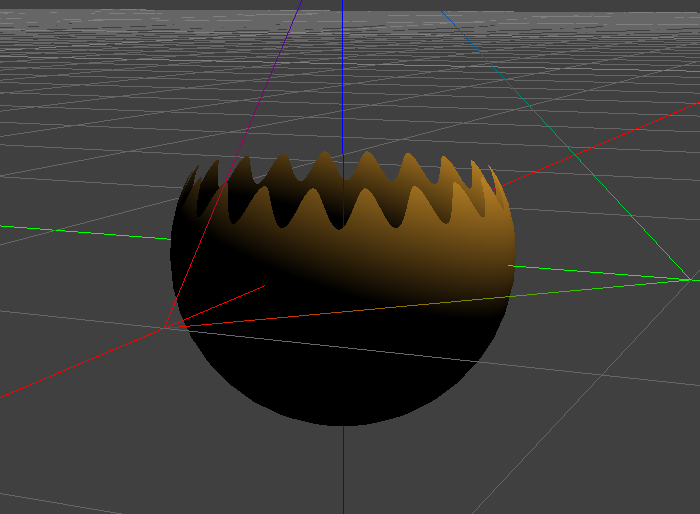
\includegraphics[width=\textwidth]{images/custom-function-node-effect.png}
    \caption{Custom Function Node example effect.}
    \label{fig:custom-function-node-example}
\end{figure}

\chapter{Remap Node in AGE}\label{app:remap-node}
The following is a possible implementation of the remap node using AGE's node library.
\begin{minted}{cpp}
// x - input_min
auto x_minus_in_min = sgraph->insert<SubtractNode>(SCALAR);
// connect(dst_node, dst_slot, src_node, src_slot)
sgraph->connect(x_minus_in_min, 0, x, 0);
sgraph->connect(x_minus_in_min, 1, input_min, 0);
// input_max - input_min
auto in_range = sgraph->insert<SubtractNode>(SCALAR);
sgraph->connect(in_range, 0, input_max, 0);
sgraph->connect(in_range, 1, input_min, 0);
// (x - input_min)/(input_max - input_min)
auto normalized_x = sgraph->insert<DivideNode>(SCALAR);
sgraph->connect(normalized_x, 0, x_minus_in_min, 0);
sgraph->connect(normalized_x, 1, in_range, 0);
// output_max - output_min
auto out_range = sgraph->insert<SubtractNode>(SCALAR);
sgraph->connect(out_range, 0, output_max, 0);
sgraph->connect(out_range, 1, output_min, 0);
// ((x - input_min)/(input_max - input_min))
//     *(output_max - output_min)
auto rescaled_x = sgraph->insert<MultiplyNode>(SCALAR);
sgraph->connect(rescaled_x, 0, normalized_x, 0);
sgraph->connect(rescaled_x, 1, out_range, 0);
// ((x - input_min)/(input_max - input_min))
//     *(output_max - output_min) + output_min
auto remapped_x = sgraph->insert<AddNode>(SCALAR);
sgraph->connect(remapped_x, 0, rescaled_x, 0);
sgraph->connect(remapped_x, 1, output_min, 0);
\end{minted}

\chapter{Attachments}\label{app:attachments}
This thesis has two attachments. The first is the \verb|measurements/| directory containing the
data used in the performance evaluation of the shader graph (see Chapter~\ref{chap:performance-evaluation}).

The second is the \verb|application/| folder retaining the source code of an application that 
presents the shader graph’s essential use cases and serves as a guide for its utilization in material creation.
It contains a series of example scenes demonstrating the shader graph’s
feature set, including the scenes used for performance evaluation.
Instructions on how to build, run, and use the application are included in the \verb|application/README.md| file.

\end{document}
